\documentclass[12pt,a4paper]{article}
\usepackage[T1]{fontenc}
\usepackage{mathptmx}
\usepackage[margin=25mm]{geometry}
\usepackage{amsmath}
\usepackage{graphicx}
\usepackage{textcomp}
\usepackage{booktabs}
\usepackage{array}
\usepackage{url}
\usepackage[hidelinks]{hyperref}
\usepackage{caption}
\usepackage{fancyhdr}
\captionsetup{font=small,labelfont=bf,labelsep=period,justification=raggedright,singlelinecheck=false}
\newcolumntype{L}[1]{>{\raggedright\arraybackslash}p{#1}}
\newcommand{\botrule}{\bottomrule}
\newcommand{\tabnote}[1]{\par\vspace{2pt}{\footnotesize\raggedright #1\par}}
\pagestyle{fancy}\fancyhf{}\renewcommand{\headrulewidth}{0pt}
\fancyhead[R]{\small Testing what a score measures}\fancyfoot[C]{\thepage}
\raggedbottom
\setlength{\parskip}{0pt}
% Generated by evaluation/summarise.mjs from evaluation/results. Do not edit by hand.
\newcommand{\BaseFuncCorePassed}{31}
\newcommand{\BaseFuncSafePassed}{2}
\newcommand{\BaseFuncAllPassed}{33}
\newcommand{\BaseLatRegisterMedian}{478.3}
\newcommand{\BaseLatRegisterPninetyfive}{542.9}
\newcommand{\BaseLatLoginMedian}{477.5}
\newcommand{\BaseLatLoginPninetyfive}{545.7}
\newcommand{\BaseLatLogadecisionMedian}{8.6}
\newcommand{\BaseLatLogadecisionPninetyfive}{16.5}
\newcommand{\BaseLatRecordanoutcomeMedian}{12.0}
\newcommand{\BaseLatRecordanoutcomePninetyfive}{19.9}
\newcommand{\BaseLatListdecisionsThreeZerodecisionsMedian}{7.2}
\newcommand{\BaseLatListdecisionsThreeZerodecisionsPninetyfive}{12.8}
\newcommand{\BaseLatViewonedecisionMedian}{8.7}
\newcommand{\BaseLatViewonedecisionPninetyfive}{13.6}
\newcommand{\BaseLatExportareportMedian}{6.8}
\newcommand{\BaseLatExportareportPninetyfive}{12.3}
\newcommand{\BaseAnalyticsOneZeroMedian}{20.1}
\newcommand{\BaseAnalyticsOneZeroPninetyfive}{30.4}
\newcommand{\BaseSnapshotsOneZero}{31}
\newcommand{\BaseAnalyticsFiveZeroMedian}{45.7}
\newcommand{\BaseAnalyticsFiveZeroPninetyfive}{74.3}
\newcommand{\BaseSnapshotsFiveZero}{31}
\newcommand{\BaseAnalyticsOneZeroZeroMedian}{79.1}
\newcommand{\BaseAnalyticsOneZeroZeroPninetyfive}{102.7}
\newcommand{\BaseSnapshotsOneZeroZero}{31}
\newcommand{\BaseAnalyticsTwoFiveZeroMedian}{192.7}
\newcommand{\BaseAnalyticsTwoFiveZeroPninetyfive}{272.8}
\newcommand{\BaseSnapshotsTwoFiveZero}{31}
\newcommand{\BaseAnalyticsFiveZeroZeroMedian}{402.7}
\newcommand{\BaseAnalyticsFiveZeroZeroPninetyfive}{505.0}
\newcommand{\BaseSnapshotsFiveZeroZero}{31}
\newcommand{\BaseAnalyticsOneZeroZeroZeroMedian}{924.1}
\newcommand{\BaseAnalyticsOneZeroZeroZeroPninetyfive}{1107.6}
\newcommand{\BaseSnapshotsOneZeroZeroZero}{31}
\newcommand{\BaseDashboardOneZeroMedian}{30.4}
\newcommand{\BaseDashboardOneZeroPninetyfive}{56.7}
\newcommand{\BaseDashboardFiveZeroMedian}{64.9}
\newcommand{\BaseDashboardFiveZeroPninetyfive}{92.4}
\newcommand{\BaseDashboardOneZeroZeroMedian}{106.8}
\newcommand{\BaseDashboardOneZeroZeroPninetyfive}{152.0}
\newcommand{\BaseDashboardTwoFiveZeroMedian}{219.1}
\newcommand{\BaseDashboardTwoFiveZeroPninetyfive}{323.0}
\newcommand{\BaseDashboardFiveZeroZeroMedian}{458.0}
\newcommand{\BaseDashboardFiveZeroZeroPninetyfive}{653.0}
\newcommand{\BaseDashboardOneZeroZeroZeroMedian}{975.3}
\newcommand{\BaseDashboardOneZeroZeroZeroPninetyfive}{1249.2}
\newcommand{\BaseStatementsTwoZero}{22}
\newcommand{\BaseStatementsOneZeroZero}{102}
\newcommand{\BaseStatementsFiveZeroZero}{502}
\newcommand{\BaseDashStatementsTwoZero}{22}
\newcommand{\BaseDashStatementsOneZeroZero}{102}
\newcommand{\BaseDashStatementsFiveZeroZero}{502}
\newcommand{\BaseLoadOneZeroZeroRequests}{196}
\newcommand{\BaseLoadOneZeroZeroThroughput}{9.8}
\newcommand{\BaseLoadOneZeroZeroMedian}{1025.0}
\newcommand{\BaseLoadOneZeroZeroPninetyfive}{1236.9}
\newcommand{\BaseLoadOneZeroZeroErrors}{0}
\newcommand{\BaseLoadFiveZeroZeroRequests}{49}
\newcommand{\BaseLoadFiveZeroZeroThroughput}{2.5}
\newcommand{\BaseLoadFiveZeroZeroMedian}{4744.9}
\newcommand{\BaseLoadFiveZeroZeroPninetyfive}{5124.7}
\newcommand{\BaseLoadFiveZeroZeroErrors}{0}
\newcommand{\BaseRttZeroAnalytics}{107.5}
\newcommand{\BaseRttZeroDashboard}{129.3}
\newcommand{\BaseRttTwoAnalytics}{118.3}
\newcommand{\BaseRttTwoDashboard}{126.9}
\newcommand{\BaseRttFiveAnalytics}{147.2}
\newcommand{\BaseRttFiveDashboard}{172.7}
\newcommand{\BaseRttOneZeroAnalytics}{195.9}
\newcommand{\BaseRttOneZeroDashboard}{209.6}
\newcommand{\BaseRttTwoZeroAnalytics}{295.0}
\newcommand{\BaseRttTwoZeroDashboard}{314.9}
\newcommand{\BaseDiffMismatches}{0}
\newcommand{\BaseDiffCompared}{606}
\newcommand{\BaseSimCalibratedmeanGap}{-0.0}
\newcommand{\BaseSimCalibratedmeanGapSD}{0.2}
\newcommand{\BaseSimCalibrateddecisionAccuracyScore}{86.2}
\newcommand{\BaseSimCalibrateddecisionAccuracyScoreSD}{1.8}
\newcommand{\BaseSimCalibratedconfidenceCalibrationScore}{98.2}
\newcommand{\BaseSimCalibratedconfidenceCalibrationScoreSD}{1.4}
\newcommand{\BaseSimCalibratedriskCalibrationScore}{57.7}
\newcommand{\BaseSimCalibratedriskCalibrationScoreSD}{2.9}
\newcommand{\BaseSimCalibratedemotionalBiasScore}{0.0}
\newcommand{\BaseSimCalibratedemotionalBiasScoreSD}{0.0}
\newcommand{\BaseSimCalibratedoverconfidenceRate}{20.2}
\newcommand{\BaseSimCalibratedoverconfidenceRateSD}{4.7}
\newcommand{\BaseSimCalibratedunderconfidenceRate}{20.8}
\newcommand{\BaseSimCalibratedunderconfidenceRateSD}{6.8}
\newcommand{\BaseSimOverconfidentmeanGap}{1.9}
\newcommand{\BaseSimOverconfidentmeanGapSD}{0.2}
\newcommand{\BaseSimOverconfidentdecisionAccuracyScore}{79.2}
\newcommand{\BaseSimOverconfidentdecisionAccuracyScoreSD}{2.4}
\newcommand{\BaseSimOverconfidentconfidenceCalibrationScore}{81.4}
\newcommand{\BaseSimOverconfidentconfidenceCalibrationScoreSD}{2.5}
\newcommand{\BaseSimOverconfidentriskCalibrationScore}{57.7}
\newcommand{\BaseSimOverconfidentriskCalibrationScoreSD}{2.9}
\newcommand{\BaseSimOverconfidentemotionalBiasScore}{0.0}
\newcommand{\BaseSimOverconfidentemotionalBiasScoreSD}{0.0}
\newcommand{\BaseSimOverconfidentoverconfidenceRate}{58.0}
\newcommand{\BaseSimOverconfidentoverconfidenceRateSD}{7.9}
\newcommand{\BaseSimOverconfidentunderconfidenceRate}{2.5}
\newcommand{\BaseSimOverconfidentunderconfidenceRateSD}{2.2}
\newcommand{\BaseSimUnderconfidentmeanGap}{-1.9}
\newcommand{\BaseSimUnderconfidentmeanGapSD}{0.2}
\newcommand{\BaseSimUnderconfidentdecisionAccuracyScore}{78.4}
\newcommand{\BaseSimUnderconfidentdecisionAccuracyScoreSD}{1.9}
\newcommand{\BaseSimUnderconfidentconfidenceCalibrationScore}{80.6}
\newcommand{\BaseSimUnderconfidentconfidenceCalibrationScoreSD}{2.4}
\newcommand{\BaseSimUnderconfidentriskCalibrationScore}{57.7}
\newcommand{\BaseSimUnderconfidentriskCalibrationScoreSD}{2.9}
\newcommand{\BaseSimUnderconfidentemotionalBiasScore}{0.0}
\newcommand{\BaseSimUnderconfidentemotionalBiasScoreSD}{0.0}
\newcommand{\BaseSimUnderconfidentoverconfidenceRate}{2.8}
\newcommand{\BaseSimUnderconfidentoverconfidenceRateSD}{2.7}
\newcommand{\BaseSimUnderconfidentunderconfidenceRate}{59.9}
\newcommand{\BaseSimUnderconfidentunderconfidenceRateSD}{6.6}
\newcommand{\BaseSimInconsistentmeanGap}{-0.1}
\newcommand{\BaseSimInconsistentmeanGapSD}{0.2}
\newcommand{\BaseSimInconsistentdecisionAccuracyScore}{75.1}
\newcommand{\BaseSimInconsistentdecisionAccuracyScoreSD}{2.1}
\newcommand{\BaseSimInconsistentconfidenceCalibrationScore}{98.2}
\newcommand{\BaseSimInconsistentconfidenceCalibrationScoreSD}{1.8}
\newcommand{\BaseSimInconsistentriskCalibrationScore}{57.7}
\newcommand{\BaseSimInconsistentriskCalibrationScoreSD}{2.9}
\newcommand{\BaseSimInconsistentemotionalBiasScore}{0.0}
\newcommand{\BaseSimInconsistentemotionalBiasScoreSD}{0.0}
\newcommand{\BaseSimInconsistentoverconfidenceRate}{32.2}
\newcommand{\BaseSimInconsistentoverconfidenceRateSD}{5.4}
\newcommand{\BaseSimInconsistentunderconfidenceRate}{35.0}
\newcommand{\BaseSimInconsistentunderconfidenceRateSD}{4.6}
\newcommand{\BaseWorkeddecisionAccuracyScore}{77}
\newcommand{\BaseWorkedriskCalibrationScore}{56}
\newcommand{\BaseWorkedemotionalBiasScore}{18}
\newcommand{\BaseWorkedconfidenceCalibrationScore}{91}
\newcommand{\BaseWorkedtotalDecisions}{10}
\newcommand{\BaseWorkedpendingDecisions}{0}
\newcommand{\BaseWorkedcompletedDecisions}{10}
\newcommand{\BaseWorkedoverconfidenceRate}{40}
\newcommand{\BaseWorkedunderconfidenceRate}{20}
\newcommand{\BaseWorkedhighRiskSuccessRate}{35}
\newcommand{\BaseWorkedlowRiskSuccessRate}{77}
\newcommand{\RevFuncCorePassed}{33}
\newcommand{\RevFuncSafePassed}{13}
\newcommand{\RevFuncAllPassed}{46}
\newcommand{\RevLatRegisterMedian}{464.3}
\newcommand{\RevLatRegisterPninetyfive}{553.7}
\newcommand{\RevLatLoginMedian}{458.1}
\newcommand{\RevLatLoginPninetyfive}{505.8}
\newcommand{\RevLatLogadecisionMedian}{8.6}
\newcommand{\RevLatLogadecisionPninetyfive}{11.6}
\newcommand{\RevLatRecordanoutcomeMedian}{8.9}
\newcommand{\RevLatRecordanoutcomePninetyfive}{12.5}
\newcommand{\RevLatListdecisionsThreeZerodecisionsMedian}{5.5}
\newcommand{\RevLatListdecisionsThreeZerodecisionsPninetyfive}{10.6}
\newcommand{\RevLatViewonedecisionMedian}{5.3}
\newcommand{\RevLatViewonedecisionPninetyfive}{9.9}
\newcommand{\RevLatExportareportMedian}{5.8}
\newcommand{\RevLatExportareportPninetyfive}{14.3}
\newcommand{\RevAnalyticsOneZeroMedian}{9.8}
\newcommand{\RevAnalyticsOneZeroPninetyfive}{18.3}
\newcommand{\RevSnapshotsOneZero}{1}
\newcommand{\RevAnalyticsFiveZeroMedian}{8.7}
\newcommand{\RevAnalyticsFiveZeroPninetyfive}{14.0}
\newcommand{\RevSnapshotsFiveZero}{1}
\newcommand{\RevAnalyticsOneZeroZeroMedian}{10.0}
\newcommand{\RevAnalyticsOneZeroZeroPninetyfive}{19.2}
\newcommand{\RevSnapshotsOneZeroZero}{1}
\newcommand{\RevAnalyticsTwoFiveZeroMedian}{16.3}
\newcommand{\RevAnalyticsTwoFiveZeroPninetyfive}{37.7}
\newcommand{\RevSnapshotsTwoFiveZero}{1}
\newcommand{\RevAnalyticsFiveZeroZeroMedian}{21.8}
\newcommand{\RevAnalyticsFiveZeroZeroPninetyfive}{36.2}
\newcommand{\RevSnapshotsFiveZeroZero}{1}
\newcommand{\RevAnalyticsOneZeroZeroZeroMedian}{36.7}
\newcommand{\RevAnalyticsOneZeroZeroZeroPninetyfive}{71.1}
\newcommand{\RevSnapshotsOneZeroZeroZero}{1}
\newcommand{\RevDashboardOneZeroMedian}{18.3}
\newcommand{\RevDashboardOneZeroPninetyfive}{49.0}
\newcommand{\RevDashboardFiveZeroMedian}{19.1}
\newcommand{\RevDashboardFiveZeroPninetyfive}{26.9}
\newcommand{\RevDashboardOneZeroZeroMedian}{22.5}
\newcommand{\RevDashboardOneZeroZeroPninetyfive}{36.1}
\newcommand{\RevDashboardTwoFiveZeroMedian}{33.0}
\newcommand{\RevDashboardTwoFiveZeroPninetyfive}{50.4}
\newcommand{\RevDashboardFiveZeroZeroMedian}{50.2}
\newcommand{\RevDashboardFiveZeroZeroPninetyfive}{93.3}
\newcommand{\RevDashboardOneZeroZeroZeroMedian}{79.4}
\newcommand{\RevDashboardOneZeroZeroZeroPninetyfive}{122.6}
\newcommand{\RevStatementsTwoZero}{2}
\newcommand{\RevStatementsOneZeroZero}{2}
\newcommand{\RevStatementsFiveZeroZero}{2}
\newcommand{\RevDashStatementsTwoZero}{3}
\newcommand{\RevDashStatementsOneZeroZero}{3}
\newcommand{\RevDashStatementsFiveZeroZero}{3}
\newcommand{\RevLoadOneZeroZeroRequests}{2,584}
\newcommand{\RevLoadOneZeroZeroThroughput}{129.2}
\newcommand{\RevLoadOneZeroZeroMedian}{71.7}
\newcommand{\RevLoadOneZeroZeroPninetyfive}{109.6}
\newcommand{\RevLoadOneZeroZeroErrors}{0}
\newcommand{\RevLoadFiveZeroZeroRequests}{1,074}
\newcommand{\RevLoadFiveZeroZeroThroughput}{53.7}
\newcommand{\RevLoadFiveZeroZeroMedian}{175.7}
\newcommand{\RevLoadFiveZeroZeroPninetyfive}{266.1}
\newcommand{\RevLoadFiveZeroZeroErrors}{0}
\newcommand{\RevRttZeroAnalytics}{17.3}
\newcommand{\RevRttZeroDashboard}{32.9}
\newcommand{\RevRttTwoAnalytics}{21.4}
\newcommand{\RevRttTwoDashboard}{36.2}
\newcommand{\RevRttFiveAnalytics}{28.4}
\newcommand{\RevRttFiveDashboard}{51.1}
\newcommand{\RevRttOneZeroAnalytics}{38.1}
\newcommand{\RevRttOneZeroDashboard}{58.7}
\newcommand{\RevRttTwoZeroAnalytics}{59.8}
\newcommand{\RevRttTwoZeroDashboard}{95.6}
\newcommand{\RevDiffMismatches}{0}
\newcommand{\RevDiffCompared}{606}
\newcommand{\RevSimCalibratedmeanGap}{-0.0}
\newcommand{\RevSimCalibratedmeanGapSD}{0.2}
\newcommand{\RevSimCalibrateddecisionAccuracyScore}{86.2}
\newcommand{\RevSimCalibrateddecisionAccuracyScoreSD}{1.8}
\newcommand{\RevSimCalibratedconfidenceCalibrationScore}{93.3}
\newcommand{\RevSimCalibratedconfidenceCalibrationScoreSD}{1.6}
\newcommand{\RevSimCalibratedriskCalibrationScore}{97.0}
\newcommand{\RevSimCalibratedriskCalibrationScoreSD}{1.4}
\newcommand{\RevSimCalibratedemotionalBiasScore}{0.0}
\newcommand{\RevSimCalibratedemotionalBiasScoreSD}{0.0}
\newcommand{\RevSimCalibratedoverconfidenceRate}{20.2}
\newcommand{\RevSimCalibratedoverconfidenceRateSD}{4.7}
\newcommand{\RevSimCalibratedunderconfidenceRate}{20.8}
\newcommand{\RevSimCalibratedunderconfidenceRateSD}{6.8}
\newcommand{\RevSimOverconfidentmeanGap}{1.9}
\newcommand{\RevSimOverconfidentmeanGapSD}{0.2}
\newcommand{\RevSimOverconfidentdecisionAccuracyScore}{79.2}
\newcommand{\RevSimOverconfidentdecisionAccuracyScoreSD}{2.4}
\newcommand{\RevSimOverconfidentconfidenceCalibrationScore}{81.1}
\newcommand{\RevSimOverconfidentconfidenceCalibrationScoreSD}{2.4}
\newcommand{\RevSimOverconfidentriskCalibrationScore}{81.4}
\newcommand{\RevSimOverconfidentriskCalibrationScoreSD}{2.5}
\newcommand{\RevSimOverconfidentemotionalBiasScore}{0.0}
\newcommand{\RevSimOverconfidentemotionalBiasScoreSD}{0.0}
\newcommand{\RevSimOverconfidentoverconfidenceRate}{58.0}
\newcommand{\RevSimOverconfidentoverconfidenceRateSD}{7.9}
\newcommand{\RevSimOverconfidentunderconfidenceRate}{2.5}
\newcommand{\RevSimOverconfidentunderconfidenceRateSD}{2.2}
\newcommand{\RevSimUnderconfidentmeanGap}{-1.9}
\newcommand{\RevSimUnderconfidentmeanGapSD}{0.2}
\newcommand{\RevSimUnderconfidentdecisionAccuracyScore}{78.4}
\newcommand{\RevSimUnderconfidentdecisionAccuracyScoreSD}{1.9}
\newcommand{\RevSimUnderconfidentconfidenceCalibrationScore}{80.3}
\newcommand{\RevSimUnderconfidentconfidenceCalibrationScoreSD}{2.4}
\newcommand{\RevSimUnderconfidentriskCalibrationScore}{80.6}
\newcommand{\RevSimUnderconfidentriskCalibrationScoreSD}{2.4}
\newcommand{\RevSimUnderconfidentemotionalBiasScore}{0.0}
\newcommand{\RevSimUnderconfidentemotionalBiasScoreSD}{0.0}
\newcommand{\RevSimUnderconfidentoverconfidenceRate}{2.8}
\newcommand{\RevSimUnderconfidentoverconfidenceRateSD}{2.7}
\newcommand{\RevSimUnderconfidentunderconfidenceRate}{59.9}
\newcommand{\RevSimUnderconfidentunderconfidenceRateSD}{6.6}
\newcommand{\RevSimInconsistentmeanGap}{-0.1}
\newcommand{\RevSimInconsistentmeanGapSD}{0.2}
\newcommand{\RevSimInconsistentdecisionAccuracyScore}{75.1}
\newcommand{\RevSimInconsistentdecisionAccuracyScoreSD}{2.1}
\newcommand{\RevSimInconsistentconfidenceCalibrationScore}{82.0}
\newcommand{\RevSimInconsistentconfidenceCalibrationScoreSD}{3.4}
\newcommand{\RevSimInconsistentriskCalibrationScore}{79.0}
\newcommand{\RevSimInconsistentriskCalibrationScoreSD}{2.0}
\newcommand{\RevSimInconsistentemotionalBiasScore}{0.0}
\newcommand{\RevSimInconsistentemotionalBiasScoreSD}{0.0}
\newcommand{\RevSimInconsistentoverconfidenceRate}{32.2}
\newcommand{\RevSimInconsistentoverconfidenceRateSD}{5.4}
\newcommand{\RevSimInconsistentunderconfidenceRate}{35.0}
\newcommand{\RevSimInconsistentunderconfidenceRateSD}{4.6}
\newcommand{\RevWorkeddecisionAccuracyScore}{77}
\newcommand{\RevWorkedriskCalibrationScore}{85}
\newcommand{\RevWorkedemotionalBiasScore}{26}
\newcommand{\RevWorkedconfidenceCalibrationScore}{81}
\newcommand{\RevWorkedtotalDecisions}{10}
\newcommand{\RevWorkedpendingDecisions}{0}
\newcommand{\RevWorkedcompletedDecisions}{10}
\newcommand{\RevWorkedoverconfidenceRate}{40}
\newcommand{\RevWorkedunderconfidenceRate}{20}
\newcommand{\RevWorkedhighRiskSuccessRate}{35}
\newcommand{\RevWorkedlowRiskSuccessRate}{77}
\newcommand{\RevWorkedmeanConfidenceGap}{0.9}
\newcommand{\RevWorkedcalibrationError}{1.9}
\newcommand{\RevWorkedriskCalibrationError}{1.5}
\newcommand{\RevWorkedminimumHistory}{20}
\newcommand{\AnalyticsReductionFiveZeroZero}{95}
\newcommand{\DashboardReductionFiveZeroZero}{89}
\newcommand{\AnalyticsReductionOneZeroZeroZero}{96}
\newcommand{\DashboardReductionOneZeroZeroZero}{92}
\newcommand{\LoadGainOneZeroZero}{13.2}
\newcommand{\LoadGainFiveZeroZero}{21.5}
\newcommand{\ProxyOffsetMin}{7}
\newcommand{\ProxyOffsetMax}{28}
\newcommand{\PasswordMin}{0.46}
\newcommand{\PasswordMax}{0.48}
\newcommand{\OtherEndpointMax}{12}
\newcommand{\BaseRttSlope}{9.4}
\newcommand{\RevRttSlope}{2.1}
\newcommand{\MRMROnebaselineconfidenceCalibrationScore}{0.0}
\newcommand{\MRMROnebaselineriskCalibrationScore}{100.0}
\newcommand{\MRMROnerevisedconfidenceCalibrationScore}{0.0}
\newcommand{\MRMROnerevisedriskCalibrationScore}{0.0}
\newcommand{\MRMRTwoabaselineconfidenceCalibrationScore}{14.2}
\newcommand{\MRMRTwoabaselineriskCalibrationScore}{100.0}
\newcommand{\MRMRTwoarevisedconfidenceCalibrationScore}{0.0}
\newcommand{\MRMRTwoarevisedriskCalibrationScore}{0.0}
\newcommand{\MRMRTwobbaselineconfidenceCalibrationScore}{100.0}
\newcommand{\MRMRTwobbaselineriskCalibrationScore}{100.0}
\newcommand{\MRMRTwobrevisedconfidenceCalibrationScore}{0.1}
\newcommand{\MRMRTwobrevisedriskCalibrationScore}{0.0}
\newcommand{\MRMRThreebaselineconfidenceCalibrationScore}{0.0}
\newcommand{\MRMRThreebaselineriskCalibrationScore}{100.0}
\newcommand{\MRMRThreerevisedconfidenceCalibrationScore}{0.0}
\newcommand{\MRMRThreerevisedriskCalibrationScore}{0.0}
\newcommand{\MRMRFourbaselinedecisionAccuracyScore}{0.0}
\newcommand{\MRMRFourbaselineconfidenceCalibrationScore}{0.0}
\newcommand{\MRMRFourbaselineriskCalibrationScore}{0.0}
\newcommand{\MRMRFourbaselineemotionalBiasScore}{0.0}
\newcommand{\MRMRFourreviseddecisionAccuracyScore}{0.0}
\newcommand{\MRMRFourrevisedconfidenceCalibrationScore}{0.0}
\newcommand{\MRMRFourrevisedriskCalibrationScore}{0.0}
\newcommand{\MRMRFourrevisedemotionalBiasScore}{0.0}
\newcommand{\MRMRFivebaselinedecisionAccuracyScore}{0.0}
\newcommand{\MRMRFivebaselineconfidenceCalibrationScore}{0.0}
\newcommand{\MRMRFivebaselineriskCalibrationScore}{0.0}
\newcommand{\MRMRFivebaselineemotionalBiasScore}{0.0}
\newcommand{\MRMRFivereviseddecisionAccuracyScore}{0.0}
\newcommand{\MRMRFiverevisedconfidenceCalibrationScore}{0.0}
\newcommand{\MRMRFiverevisedriskCalibrationScore}{0.0}
\newcommand{\MRMRFiverevisedemotionalBiasScore}{0.0}
\newcommand{\MRMRSixbaselinedecisionAccuracyScore}{0.0}
\newcommand{\MRMRSixbaselineconfidenceCalibrationScore}{0.0}
\newcommand{\MRMRSixbaselineriskCalibrationScore}{0.0}
\newcommand{\MRMRSixreviseddecisionAccuracyScore}{0.0}
\newcommand{\MRMRSixrevisedconfidenceCalibrationScore}{0.0}
\newcommand{\MRMRSixrevisedriskCalibrationScore}{0.0}
\newcommand{\MRMRSevenbaselineemotionalBiasScore}{100.0}
\newcommand{\MRMRSevenrevisedemotionalBiasScore}{0.0}
\newcommand{\MRMREightbaselineemotionalBiasScore}{100.0}
\newcommand{\MRMREightrevisedemotionalBiasScore}{0.0}
\newcommand{\MRMRNinebaselineemotionalBiasScore}{0.0}
\newcommand{\MRMRNinerevisedemotionalBiasScore}{0.0}
\newcommand{\MRSources}{1,000}
\newcommand{\PowerReps}{1,000}
\newcommand{\MinimumHistory}{20}
\newcommand{\PowOverOneBaseCCNFiveAuc}{0.73}
\newcommand{\PowOverOneBaseCCNFiveSens}{22}
\newcommand{\PowOverOneBaseRCNFiveAuc}{0.50}
\newcommand{\PowOverOneBaseRCNFiveSens}{3}
\newcommand{\PowOverOneBaseDANFiveAuc}{0.64}
\newcommand{\PowOverOneBaseDANFiveSens}{16}
\newcommand{\PowOverOneRevCCNFiveAuc}{0.66}
\newcommand{\PowOverOneRevCCNFiveSens}{14}
\newcommand{\PowOverOneRevRCNFiveAuc}{0.68}
\newcommand{\PowOverOneRevRCNFiveSens}{18}
\newcommand{\PowOverTwoBaseCCNFiveAuc}{0.95}
\newcommand{\PowOverTwoBaseCCNFiveSens}{73}
\newcommand{\PowOverTwoBaseRCNFiveAuc}{0.50}
\newcommand{\PowOverTwoBaseRCNFiveSens}{3}
\newcommand{\PowOverTwoBaseDANFiveAuc}{0.88}
\newcommand{\PowOverTwoBaseDANFiveSens}{55}
\newcommand{\PowOverTwoRevCCNFiveAuc}{0.90}
\newcommand{\PowOverTwoRevCCNFiveSens}{53}
\newcommand{\PowOverTwoRevRCNFiveAuc}{0.92}
\newcommand{\PowOverTwoRevRCNFiveSens}{64}
\newcommand{\PowUnderTwoBaseCCNFiveAuc}{0.96}
\newcommand{\PowUnderTwoBaseCCNFiveSens}{77}
\newcommand{\PowUnderTwoBaseRCNFiveAuc}{0.50}
\newcommand{\PowUnderTwoBaseRCNFiveSens}{3}
\newcommand{\PowUnderTwoBaseDANFiveAuc}{0.90}
\newcommand{\PowUnderTwoBaseDANFiveSens}{62}
\newcommand{\PowUnderTwoRevCCNFiveAuc}{0.92}
\newcommand{\PowUnderTwoRevCCNFiveSens}{59}
\newcommand{\PowUnderTwoRevRCNFiveAuc}{0.93}
\newcommand{\PowUnderTwoRevRCNFiveSens}{69}
\newcommand{\PowIncTwoBaseCCNFiveAuc}{0.56}
\newcommand{\PowIncTwoBaseCCNFiveSens}{6}
\newcommand{\PowIncTwoBaseRCNFiveAuc}{0.50}
\newcommand{\PowIncTwoBaseRCNFiveSens}{3}
\newcommand{\PowIncTwoBaseDANFiveAuc}{0.79}
\newcommand{\PowIncTwoBaseDANFiveSens}{35}
\newcommand{\PowIncTwoRevCCNFiveAuc}{0.64}
\newcommand{\PowIncTwoRevCCNFiveSens}{13}
\newcommand{\PowIncTwoRevRCNFiveAuc}{0.82}
\newcommand{\PowIncTwoRevRCNFiveSens}{37}
\newcommand{\PowIncThreeBaseCCNFiveAuc}{0.63}
\newcommand{\PowIncThreeBaseCCNFiveSens}{10}
\newcommand{\PowIncThreeBaseRCNFiveAuc}{0.50}
\newcommand{\PowIncThreeBaseRCNFiveSens}{3}
\newcommand{\PowIncThreeBaseDANFiveAuc}{0.94}
\newcommand{\PowIncThreeBaseDANFiveSens}{73}
\newcommand{\PowIncThreeRevCCNFiveAuc}{0.87}
\newcommand{\PowIncThreeRevCCNFiveSens}{52}
\newcommand{\PowIncThreeRevRCNFiveAuc}{0.96}
\newcommand{\PowIncThreeRevRCNFiveSens}{76}
\newcommand{\PowNoisyTwoBaseCCNFiveAuc}{0.63}
\newcommand{\PowNoisyTwoBaseCCNFiveSens}{18}
\newcommand{\PowNoisyTwoBaseRCNFiveAuc}{0.50}
\newcommand{\PowNoisyTwoBaseRCNFiveSens}{3}
\newcommand{\PowNoisyTwoBaseDANFiveAuc}{0.81}
\newcommand{\PowNoisyTwoBaseDANFiveSens}{43}
\newcommand{\PowNoisyTwoRevCCNFiveAuc}{0.81}
\newcommand{\PowNoisyTwoRevCCNFiveSens}{36}
\newcommand{\PowNoisyTwoRevRCNFiveAuc}{0.76}
\newcommand{\PowNoisyTwoRevRCNFiveSens}{33}
\newcommand{\PowOverOneBaseCCNOneZeroAuc}{0.83}
\newcommand{\PowOverOneBaseCCNOneZeroSens}{46}
\newcommand{\PowOverOneBaseRCNOneZeroAuc}{0.50}
\newcommand{\PowOverOneBaseRCNOneZeroSens}{4}
\newcommand{\PowOverOneBaseDANOneZeroAuc}{0.69}
\newcommand{\PowOverOneBaseDANOneZeroSens}{20}
\newcommand{\PowOverOneRevCCNOneZeroAuc}{0.74}
\newcommand{\PowOverOneRevCCNOneZeroSens}{28}
\newcommand{\PowOverOneRevRCNOneZeroAuc}{0.78}
\newcommand{\PowOverOneRevRCNOneZeroSens}{43}
\newcommand{\PowOverTwoBaseCCNOneZeroAuc}{1.00}
\newcommand{\PowOverTwoBaseCCNOneZeroSens}{96}
\newcommand{\PowOverTwoBaseRCNOneZeroAuc}{0.50}
\newcommand{\PowOverTwoBaseRCNOneZeroSens}{4}
\newcommand{\PowOverTwoBaseDANOneZeroAuc}{0.94}
\newcommand{\PowOverTwoBaseDANOneZeroSens}{72}
\newcommand{\PowOverTwoRevCCNOneZeroAuc}{0.97}
\newcommand{\PowOverTwoRevCCNOneZeroSens}{84}
\newcommand{\PowOverTwoRevRCNOneZeroAuc}{0.99}
\newcommand{\PowOverTwoRevRCNOneZeroSens}{94}
\newcommand{\PowUnderTwoBaseCCNOneZeroAuc}{0.99}
\newcommand{\PowUnderTwoBaseCCNOneZeroSens}{97}
\newcommand{\PowUnderTwoBaseRCNOneZeroAuc}{0.50}
\newcommand{\PowUnderTwoBaseRCNOneZeroSens}{4}
\newcommand{\PowUnderTwoBaseDANOneZeroAuc}{0.95}
\newcommand{\PowUnderTwoBaseDANOneZeroSens}{76}
\newcommand{\PowUnderTwoRevCCNOneZeroAuc}{0.98}
\newcommand{\PowUnderTwoRevCCNOneZeroSens}{87}
\newcommand{\PowUnderTwoRevRCNOneZeroAuc}{0.99}
\newcommand{\PowUnderTwoRevRCNOneZeroSens}{95}
\newcommand{\PowIncTwoBaseCCNOneZeroAuc}{0.52}
\newcommand{\PowIncTwoBaseCCNOneZeroSens}{6}
\newcommand{\PowIncTwoBaseRCNOneZeroAuc}{0.50}
\newcommand{\PowIncTwoBaseRCNOneZeroSens}{4}
\newcommand{\PowIncTwoBaseDANOneZeroAuc}{0.91}
\newcommand{\PowIncTwoBaseDANOneZeroSens}{56}
\newcommand{\PowIncTwoRevCCNOneZeroAuc}{0.65}
\newcommand{\PowIncTwoRevCCNOneZeroSens}{19}
\newcommand{\PowIncTwoRevRCNOneZeroAuc}{0.97}
\newcommand{\PowIncTwoRevRCNOneZeroSens}{86}
\newcommand{\PowIncThreeBaseCCNOneZeroAuc}{0.55}
\newcommand{\PowIncThreeBaseCCNOneZeroSens}{8}
\newcommand{\PowIncThreeBaseRCNOneZeroAuc}{0.50}
\newcommand{\PowIncThreeBaseRCNOneZeroSens}{4}
\newcommand{\PowIncThreeBaseDANOneZeroAuc}{0.99}
\newcommand{\PowIncThreeBaseDANOneZeroSens}{95}
\newcommand{\PowIncThreeRevCCNOneZeroAuc}{0.95}
\newcommand{\PowIncThreeRevCCNOneZeroSens}{81}
\newcommand{\PowIncThreeRevRCNOneZeroAuc}{1.00}
\newcommand{\PowIncThreeRevRCNOneZeroSens}{100}
\newcommand{\PowNoisyTwoBaseCCNOneZeroAuc}{0.62}
\newcommand{\PowNoisyTwoBaseCCNOneZeroSens}{18}
\newcommand{\PowNoisyTwoBaseRCNOneZeroAuc}{0.50}
\newcommand{\PowNoisyTwoBaseRCNOneZeroSens}{4}
\newcommand{\PowNoisyTwoBaseDANOneZeroAuc}{0.90}
\newcommand{\PowNoisyTwoBaseDANOneZeroSens}{60}
\newcommand{\PowNoisyTwoRevCCNOneZeroAuc}{0.90}
\newcommand{\PowNoisyTwoRevCCNOneZeroSens}{62}
\newcommand{\PowNoisyTwoRevRCNOneZeroAuc}{0.75}
\newcommand{\PowNoisyTwoRevRCNOneZeroSens}{37}
\newcommand{\PowOverOneBaseCCNOneFiveAuc}{0.92}
\newcommand{\PowOverOneBaseCCNOneFiveSens}{69}
\newcommand{\PowOverOneBaseRCNOneFiveAuc}{0.50}
\newcommand{\PowOverOneBaseRCNOneFiveSens}{5}
\newcommand{\PowOverOneBaseDANOneFiveAuc}{0.73}
\newcommand{\PowOverOneBaseDANOneFiveSens}{22}
\newcommand{\PowOverOneRevCCNOneFiveAuc}{0.81}
\newcommand{\PowOverOneRevCCNOneFiveSens}{38}
\newcommand{\PowOverOneRevRCNOneFiveAuc}{0.86}
\newcommand{\PowOverOneRevRCNOneFiveSens}{53}
\newcommand{\PowOverTwoBaseCCNOneFiveAuc}{1.00}
\newcommand{\PowOverTwoBaseCCNOneFiveSens}{100}
\newcommand{\PowOverTwoBaseRCNOneFiveAuc}{0.50}
\newcommand{\PowOverTwoBaseRCNOneFiveSens}{5}
\newcommand{\PowOverTwoBaseDANOneFiveAuc}{0.98}
\newcommand{\PowOverTwoBaseDANOneFiveSens}{86}
\newcommand{\PowOverTwoRevCCNOneFiveAuc}{1.00}
\newcommand{\PowOverTwoRevCCNOneFiveSens}{98}
\newcommand{\PowOverTwoRevRCNOneFiveAuc}{1.00}
\newcommand{\PowOverTwoRevRCNOneFiveSens}{100}
\newcommand{\PowUnderTwoBaseCCNOneFiveAuc}{1.00}
\newcommand{\PowUnderTwoBaseCCNOneFiveSens}{100}
\newcommand{\PowUnderTwoBaseRCNOneFiveAuc}{0.50}
\newcommand{\PowUnderTwoBaseRCNOneFiveSens}{5}
\newcommand{\PowUnderTwoBaseDANOneFiveAuc}{0.98}
\newcommand{\PowUnderTwoBaseDANOneFiveSens}{89}
\newcommand{\PowUnderTwoRevCCNOneFiveAuc}{1.00}
\newcommand{\PowUnderTwoRevCCNOneFiveSens}{98}
\newcommand{\PowUnderTwoRevRCNOneFiveAuc}{1.00}
\newcommand{\PowUnderTwoRevRCNOneFiveSens}{99}
\newcommand{\PowIncTwoBaseCCNOneFiveAuc}{0.50}
\newcommand{\PowIncTwoBaseCCNOneFiveSens}{5}
\newcommand{\PowIncTwoBaseRCNOneFiveAuc}{0.50}
\newcommand{\PowIncTwoBaseRCNOneFiveSens}{5}
\newcommand{\PowIncTwoBaseDANOneFiveAuc}{0.94}
\newcommand{\PowIncTwoBaseDANOneFiveSens}{69}
\newcommand{\PowIncTwoRevCCNOneFiveAuc}{0.63}
\newcommand{\PowIncTwoRevCCNOneFiveSens}{16}
\newcommand{\PowIncTwoRevRCNOneFiveAuc}{0.99}
\newcommand{\PowIncTwoRevRCNOneFiveSens}{95}
\newcommand{\PowIncThreeBaseCCNOneFiveAuc}{0.50}
\newcommand{\PowIncThreeBaseCCNOneFiveSens}{5}
\newcommand{\PowIncThreeBaseRCNOneFiveAuc}{0.50}
\newcommand{\PowIncThreeBaseRCNOneFiveSens}{5}
\newcommand{\PowIncThreeBaseDANOneFiveAuc}{1.00}
\newcommand{\PowIncThreeBaseDANOneFiveSens}{99}
\newcommand{\PowIncThreeRevCCNOneFiveAuc}{0.97}
\newcommand{\PowIncThreeRevCCNOneFiveSens}{88}
\newcommand{\PowIncThreeRevRCNOneFiveAuc}{1.00}
\newcommand{\PowIncThreeRevRCNOneFiveSens}{100}
\newcommand{\PowNoisyTwoBaseCCNOneFiveAuc}{0.62}
\newcommand{\PowNoisyTwoBaseCCNOneFiveSens}{23}
\newcommand{\PowNoisyTwoBaseRCNOneFiveAuc}{0.50}
\newcommand{\PowNoisyTwoBaseRCNOneFiveSens}{5}
\newcommand{\PowNoisyTwoBaseDANOneFiveAuc}{0.94}
\newcommand{\PowNoisyTwoBaseDANOneFiveSens}{74}
\newcommand{\PowNoisyTwoRevCCNOneFiveAuc}{0.95}
\newcommand{\PowNoisyTwoRevCCNOneFiveSens}{77}
\newcommand{\PowNoisyTwoRevRCNOneFiveAuc}{0.76}
\newcommand{\PowNoisyTwoRevRCNOneFiveSens}{37}
\newcommand{\PowOverOneBaseCCNTwoZeroAuc}{0.95}
\newcommand{\PowOverOneBaseCCNTwoZeroSens}{82}
\newcommand{\PowOverOneBaseRCNTwoZeroAuc}{0.50}
\newcommand{\PowOverOneBaseRCNTwoZeroSens}{3}
\newcommand{\PowOverOneBaseDANTwoZeroAuc}{0.77}
\newcommand{\PowOverOneBaseDANTwoZeroSens}{25}
\newcommand{\PowOverOneRevCCNTwoZeroAuc}{0.87}
\newcommand{\PowOverOneRevCCNTwoZeroSens}{53}
\newcommand{\PowOverOneRevRCNTwoZeroAuc}{0.92}
\newcommand{\PowOverOneRevRCNTwoZeroSens}{65}
\newcommand{\PowOverTwoBaseCCNTwoZeroAuc}{1.00}
\newcommand{\PowOverTwoBaseCCNTwoZeroSens}{100}
\newcommand{\PowOverTwoBaseRCNTwoZeroAuc}{0.50}
\newcommand{\PowOverTwoBaseRCNTwoZeroSens}{3}
\newcommand{\PowOverTwoBaseDANTwoZeroAuc}{0.99}
\newcommand{\PowOverTwoBaseDANTwoZeroSens}{93}
\newcommand{\PowOverTwoRevCCNTwoZeroAuc}{1.00}
\newcommand{\PowOverTwoRevCCNTwoZeroSens}{100}
\newcommand{\PowOverTwoRevRCNTwoZeroAuc}{1.00}
\newcommand{\PowOverTwoRevRCNTwoZeroSens}{100}
\newcommand{\PowUnderTwoBaseCCNTwoZeroAuc}{1.00}
\newcommand{\PowUnderTwoBaseCCNTwoZeroSens}{100}
\newcommand{\PowUnderTwoBaseRCNTwoZeroAuc}{0.50}
\newcommand{\PowUnderTwoBaseRCNTwoZeroSens}{3}
\newcommand{\PowUnderTwoBaseDANTwoZeroAuc}{0.99}
\newcommand{\PowUnderTwoBaseDANTwoZeroSens}{96}
\newcommand{\PowUnderTwoRevCCNTwoZeroAuc}{1.00}
\newcommand{\PowUnderTwoRevCCNTwoZeroSens}{100}
\newcommand{\PowUnderTwoRevRCNTwoZeroAuc}{1.00}
\newcommand{\PowUnderTwoRevRCNTwoZeroSens}{100}
\newcommand{\PowIncTwoBaseCCNTwoZeroAuc}{0.51}
\newcommand{\PowIncTwoBaseCCNTwoZeroSens}{7}
\newcommand{\PowIncTwoBaseRCNTwoZeroAuc}{0.50}
\newcommand{\PowIncTwoBaseRCNTwoZeroSens}{3}
\newcommand{\PowIncTwoBaseDANTwoZeroAuc}{0.96}
\newcommand{\PowIncTwoBaseDANTwoZeroSens}{80}
\newcommand{\PowIncTwoRevCCNTwoZeroAuc}{0.64}
\newcommand{\PowIncTwoRevCCNTwoZeroSens}{20}
\newcommand{\PowIncTwoRevRCNTwoZeroAuc}{1.00}
\newcommand{\PowIncTwoRevRCNTwoZeroSens}{98}
\newcommand{\PowIncThreeBaseCCNTwoZeroAuc}{0.53}
\newcommand{\PowIncThreeBaseCCNTwoZeroSens}{8}
\newcommand{\PowIncThreeBaseRCNTwoZeroAuc}{0.50}
\newcommand{\PowIncThreeBaseRCNTwoZeroSens}{3}
\newcommand{\PowIncThreeBaseDANTwoZeroAuc}{1.00}
\newcommand{\PowIncThreeBaseDANTwoZeroSens}{100}
\newcommand{\PowIncThreeRevCCNTwoZeroAuc}{0.99}
\newcommand{\PowIncThreeRevCCNTwoZeroSens}{93}
\newcommand{\PowIncThreeRevRCNTwoZeroAuc}{1.00}
\newcommand{\PowIncThreeRevRCNTwoZeroSens}{100}
\newcommand{\PowNoisyTwoBaseCCNTwoZeroAuc}{0.62}
\newcommand{\PowNoisyTwoBaseCCNTwoZeroSens}{21}
\newcommand{\PowNoisyTwoBaseRCNTwoZeroAuc}{0.50}
\newcommand{\PowNoisyTwoBaseRCNTwoZeroSens}{3}
\newcommand{\PowNoisyTwoBaseDANTwoZeroAuc}{0.97}
\newcommand{\PowNoisyTwoBaseDANTwoZeroSens}{82}
\newcommand{\PowNoisyTwoRevCCNTwoZeroAuc}{0.97}
\newcommand{\PowNoisyTwoRevCCNTwoZeroSens}{85}
\newcommand{\PowNoisyTwoRevRCNTwoZeroAuc}{0.75}
\newcommand{\PowNoisyTwoRevRCNTwoZeroSens}{32}
\newcommand{\PowOverOneBaseCCNThreeZeroAuc}{0.99}
\newcommand{\PowOverOneBaseCCNThreeZeroSens}{94}
\newcommand{\PowOverOneBaseRCNThreeZeroAuc}{0.50}
\newcommand{\PowOverOneBaseRCNThreeZeroSens}{4}
\newcommand{\PowOverOneBaseDANThreeZeroAuc}{0.82}
\newcommand{\PowOverOneBaseDANThreeZeroSens}{25}
\newcommand{\PowOverOneRevCCNThreeZeroAuc}{0.94}
\newcommand{\PowOverOneRevCCNThreeZeroSens}{65}
\newcommand{\PowOverOneRevRCNThreeZeroAuc}{0.97}
\newcommand{\PowOverOneRevRCNThreeZeroSens}{82}
\newcommand{\PowOverTwoBaseCCNThreeZeroAuc}{1.00}
\newcommand{\PowOverTwoBaseCCNThreeZeroSens}{100}
\newcommand{\PowOverTwoBaseRCNThreeZeroAuc}{0.50}
\newcommand{\PowOverTwoBaseRCNThreeZeroSens}{4}
\newcommand{\PowOverTwoBaseDANThreeZeroAuc}{1.00}
\newcommand{\PowOverTwoBaseDANThreeZeroSens}{98}
\newcommand{\PowOverTwoRevCCNThreeZeroAuc}{1.00}
\newcommand{\PowOverTwoRevCCNThreeZeroSens}{100}
\newcommand{\PowOverTwoRevRCNThreeZeroAuc}{1.00}
\newcommand{\PowOverTwoRevRCNThreeZeroSens}{100}
\newcommand{\PowUnderTwoBaseCCNThreeZeroAuc}{1.00}
\newcommand{\PowUnderTwoBaseCCNThreeZeroSens}{100}
\newcommand{\PowUnderTwoBaseRCNThreeZeroAuc}{0.50}
\newcommand{\PowUnderTwoBaseRCNThreeZeroSens}{4}
\newcommand{\PowUnderTwoBaseDANThreeZeroAuc}{1.00}
\newcommand{\PowUnderTwoBaseDANThreeZeroSens}{99}
\newcommand{\PowUnderTwoRevCCNThreeZeroAuc}{1.00}
\newcommand{\PowUnderTwoRevCCNThreeZeroSens}{100}
\newcommand{\PowUnderTwoRevRCNThreeZeroAuc}{1.00}
\newcommand{\PowUnderTwoRevRCNThreeZeroSens}{100}
\newcommand{\PowIncTwoBaseCCNThreeZeroAuc}{0.50}
\newcommand{\PowIncTwoBaseCCNThreeZeroSens}{4}
\newcommand{\PowIncTwoBaseRCNThreeZeroAuc}{0.50}
\newcommand{\PowIncTwoBaseRCNThreeZeroSens}{4}
\newcommand{\PowIncTwoBaseDANThreeZeroAuc}{0.98}
\newcommand{\PowIncTwoBaseDANThreeZeroSens}{87}
\newcommand{\PowIncTwoRevCCNThreeZeroAuc}{0.65}
\newcommand{\PowIncTwoRevCCNThreeZeroSens}{17}
\newcommand{\PowIncTwoRevRCNThreeZeroAuc}{1.00}
\newcommand{\PowIncTwoRevRCNThreeZeroSens}{100}
\newcommand{\PowIncThreeBaseCCNThreeZeroAuc}{0.50}
\newcommand{\PowIncThreeBaseCCNThreeZeroSens}{4}
\newcommand{\PowIncThreeBaseRCNThreeZeroAuc}{0.50}
\newcommand{\PowIncThreeBaseRCNThreeZeroSens}{4}
\newcommand{\PowIncThreeBaseDANThreeZeroAuc}{1.00}
\newcommand{\PowIncThreeBaseDANThreeZeroSens}{100}
\newcommand{\PowIncThreeRevCCNThreeZeroAuc}{1.00}
\newcommand{\PowIncThreeRevCCNThreeZeroSens}{97}
\newcommand{\PowIncThreeRevRCNThreeZeroAuc}{1.00}
\newcommand{\PowIncThreeRevRCNThreeZeroSens}{100}
\newcommand{\PowNoisyTwoBaseCCNThreeZeroAuc}{0.63}
\newcommand{\PowNoisyTwoBaseCCNThreeZeroSens}{21}
\newcommand{\PowNoisyTwoBaseRCNThreeZeroAuc}{0.50}
\newcommand{\PowNoisyTwoBaseRCNThreeZeroSens}{4}
\newcommand{\PowNoisyTwoBaseDANThreeZeroAuc}{0.99}
\newcommand{\PowNoisyTwoBaseDANThreeZeroSens}{88}
\newcommand{\PowNoisyTwoRevCCNThreeZeroAuc}{0.99}
\newcommand{\PowNoisyTwoRevCCNThreeZeroSens}{92}
\newcommand{\PowNoisyTwoRevRCNThreeZeroAuc}{0.75}
\newcommand{\PowNoisyTwoRevRCNThreeZeroSens}{27}
\newcommand{\PowOverOneBaseCCNFourZeroAuc}{1.00}
\newcommand{\PowOverOneBaseCCNFourZeroSens}{96}
\newcommand{\PowOverOneBaseRCNFourZeroAuc}{0.50}
\newcommand{\PowOverOneBaseRCNFourZeroSens}{3}
\newcommand{\PowOverOneBaseDANFourZeroAuc}{0.84}
\newcommand{\PowOverOneBaseDANFourZeroSens}{39}
\newcommand{\PowOverOneRevCCNFourZeroAuc}{0.98}
\newcommand{\PowOverOneRevCCNFourZeroSens}{89}
\newcommand{\PowOverOneRevRCNFourZeroAuc}{0.99}
\newcommand{\PowOverOneRevRCNFourZeroSens}{93}
\newcommand{\PowOverTwoBaseCCNFourZeroAuc}{1.00}
\newcommand{\PowOverTwoBaseCCNFourZeroSens}{100}
\newcommand{\PowOverTwoBaseRCNFourZeroAuc}{0.50}
\newcommand{\PowOverTwoBaseRCNFourZeroSens}{3}
\newcommand{\PowOverTwoBaseDANFourZeroAuc}{1.00}
\newcommand{\PowOverTwoBaseDANFourZeroSens}{100}
\newcommand{\PowOverTwoRevCCNFourZeroAuc}{1.00}
\newcommand{\PowOverTwoRevCCNFourZeroSens}{100}
\newcommand{\PowOverTwoRevRCNFourZeroAuc}{1.00}
\newcommand{\PowOverTwoRevRCNFourZeroSens}{100}
\newcommand{\PowUnderTwoBaseCCNFourZeroAuc}{1.00}
\newcommand{\PowUnderTwoBaseCCNFourZeroSens}{100}
\newcommand{\PowUnderTwoBaseRCNFourZeroAuc}{0.50}
\newcommand{\PowUnderTwoBaseRCNFourZeroSens}{3}
\newcommand{\PowUnderTwoBaseDANFourZeroAuc}{1.00}
\newcommand{\PowUnderTwoBaseDANFourZeroSens}{100}
\newcommand{\PowUnderTwoRevCCNFourZeroAuc}{1.00}
\newcommand{\PowUnderTwoRevCCNFourZeroSens}{100}
\newcommand{\PowUnderTwoRevRCNFourZeroAuc}{1.00}
\newcommand{\PowUnderTwoRevRCNFourZeroSens}{100}
\newcommand{\PowIncTwoBaseCCNFourZeroAuc}{0.49}
\newcommand{\PowIncTwoBaseCCNFourZeroSens}{2}
\newcommand{\PowIncTwoBaseRCNFourZeroAuc}{0.50}
\newcommand{\PowIncTwoBaseRCNFourZeroSens}{3}
\newcommand{\PowIncTwoBaseDANFourZeroAuc}{0.99}
\newcommand{\PowIncTwoBaseDANFourZeroSens}{96}
\newcommand{\PowIncTwoRevCCNFourZeroAuc}{0.68}
\newcommand{\PowIncTwoRevCCNFourZeroSens}{27}
\newcommand{\PowIncTwoRevRCNFourZeroAuc}{1.00}
\newcommand{\PowIncTwoRevRCNFourZeroSens}{100}
\newcommand{\PowIncThreeBaseCCNFourZeroAuc}{0.51}
\newcommand{\PowIncThreeBaseCCNFourZeroSens}{2}
\newcommand{\PowIncThreeBaseRCNFourZeroAuc}{0.50}
\newcommand{\PowIncThreeBaseRCNFourZeroSens}{3}
\newcommand{\PowIncThreeBaseDANFourZeroAuc}{1.00}
\newcommand{\PowIncThreeBaseDANFourZeroSens}{100}
\newcommand{\PowIncThreeRevCCNFourZeroAuc}{1.00}
\newcommand{\PowIncThreeRevCCNFourZeroSens}{100}
\newcommand{\PowIncThreeRevRCNFourZeroAuc}{1.00}
\newcommand{\PowIncThreeRevRCNFourZeroSens}{100}
\newcommand{\PowNoisyTwoBaseCCNFourZeroAuc}{0.64}
\newcommand{\PowNoisyTwoBaseCCNFourZeroSens}{15}
\newcommand{\PowNoisyTwoBaseRCNFourZeroAuc}{0.50}
\newcommand{\PowNoisyTwoBaseRCNFourZeroSens}{3}
\newcommand{\PowNoisyTwoBaseDANFourZeroAuc}{0.99}
\newcommand{\PowNoisyTwoBaseDANFourZeroSens}{96}
\newcommand{\PowNoisyTwoRevCCNFourZeroAuc}{1.00}
\newcommand{\PowNoisyTwoRevCCNFourZeroSens}{98}
\newcommand{\PowNoisyTwoRevRCNFourZeroAuc}{0.76}
\newcommand{\PowNoisyTwoRevRCNFourZeroSens}{28}
\newcommand{\PowOverOneBaseCCNSixZeroAuc}{1.00}
\newcommand{\PowOverOneBaseCCNSixZeroSens}{100}
\newcommand{\PowOverOneBaseRCNSixZeroAuc}{0.50}
\newcommand{\PowOverOneBaseRCNSixZeroSens}{5}
\newcommand{\PowOverOneBaseDANSixZeroAuc}{0.88}
\newcommand{\PowOverOneBaseDANSixZeroSens}{39}
\newcommand{\PowOverOneRevCCNSixZeroAuc}{0.99}
\newcommand{\PowOverOneRevCCNSixZeroSens}{98}
\newcommand{\PowOverOneRevRCNSixZeroAuc}{1.00}
\newcommand{\PowOverOneRevRCNSixZeroSens}{99}
\newcommand{\PowOverTwoBaseCCNSixZeroAuc}{1.00}
\newcommand{\PowOverTwoBaseCCNSixZeroSens}{100}
\newcommand{\PowOverTwoBaseRCNSixZeroAuc}{0.50}
\newcommand{\PowOverTwoBaseRCNSixZeroSens}{5}
\newcommand{\PowOverTwoBaseDANSixZeroAuc}{1.00}
\newcommand{\PowOverTwoBaseDANSixZeroSens}{100}
\newcommand{\PowOverTwoRevCCNSixZeroAuc}{1.00}
\newcommand{\PowOverTwoRevCCNSixZeroSens}{100}
\newcommand{\PowOverTwoRevRCNSixZeroAuc}{1.00}
\newcommand{\PowOverTwoRevRCNSixZeroSens}{100}
\newcommand{\PowUnderTwoBaseCCNSixZeroAuc}{1.00}
\newcommand{\PowUnderTwoBaseCCNSixZeroSens}{100}
\newcommand{\PowUnderTwoBaseRCNSixZeroAuc}{0.50}
\newcommand{\PowUnderTwoBaseRCNSixZeroSens}{5}
\newcommand{\PowUnderTwoBaseDANSixZeroAuc}{1.00}
\newcommand{\PowUnderTwoBaseDANSixZeroSens}{100}
\newcommand{\PowUnderTwoRevCCNSixZeroAuc}{1.00}
\newcommand{\PowUnderTwoRevCCNSixZeroSens}{100}
\newcommand{\PowUnderTwoRevRCNSixZeroAuc}{1.00}
\newcommand{\PowUnderTwoRevRCNSixZeroSens}{100}
\newcommand{\PowIncTwoBaseCCNSixZeroAuc}{0.50}
\newcommand{\PowIncTwoBaseCCNSixZeroSens}{2}
\newcommand{\PowIncTwoBaseRCNSixZeroAuc}{0.50}
\newcommand{\PowIncTwoBaseRCNSixZeroSens}{5}
\newcommand{\PowIncTwoBaseDANSixZeroAuc}{1.00}
\newcommand{\PowIncTwoBaseDANSixZeroSens}{98}
\newcommand{\PowIncTwoRevCCNSixZeroAuc}{0.72}
\newcommand{\PowIncTwoRevCCNSixZeroSens}{29}
\newcommand{\PowIncTwoRevRCNSixZeroAuc}{1.00}
\newcommand{\PowIncTwoRevRCNSixZeroSens}{100}
\newcommand{\PowIncThreeBaseCCNSixZeroAuc}{0.50}
\newcommand{\PowIncThreeBaseCCNSixZeroSens}{2}
\newcommand{\PowIncThreeBaseRCNSixZeroAuc}{0.50}
\newcommand{\PowIncThreeBaseRCNSixZeroSens}{5}
\newcommand{\PowIncThreeBaseDANSixZeroAuc}{1.00}
\newcommand{\PowIncThreeBaseDANSixZeroSens}{100}
\newcommand{\PowIncThreeRevCCNSixZeroAuc}{1.00}
\newcommand{\PowIncThreeRevCCNSixZeroSens}{100}
\newcommand{\PowIncThreeRevRCNSixZeroAuc}{1.00}
\newcommand{\PowIncThreeRevRCNSixZeroSens}{100}
\newcommand{\PowNoisyTwoBaseCCNSixZeroAuc}{0.65}
\newcommand{\PowNoisyTwoBaseCCNSixZeroSens}{14}
\newcommand{\PowNoisyTwoBaseRCNSixZeroAuc}{0.50}
\newcommand{\PowNoisyTwoBaseRCNSixZeroSens}{5}
\newcommand{\PowNoisyTwoBaseDANSixZeroAuc}{1.00}
\newcommand{\PowNoisyTwoBaseDANSixZeroSens}{99}
\newcommand{\PowNoisyTwoRevCCNSixZeroAuc}{1.00}
\newcommand{\PowNoisyTwoRevCCNSixZeroSens}{100}
\newcommand{\PowNoisyTwoRevRCNSixZeroAuc}{0.75}
\newcommand{\PowNoisyTwoRevRCNSixZeroSens}{26}
\newcommand{\PowOverOneBaseCCNEightZeroAuc}{1.00}
\newcommand{\PowOverOneBaseCCNEightZeroSens}{100}
\newcommand{\PowOverOneBaseRCNEightZeroAuc}{0.50}
\newcommand{\PowOverOneBaseRCNEightZeroSens}{4}
\newcommand{\PowOverOneBaseDANEightZeroAuc}{0.92}
\newcommand{\PowOverOneBaseDANEightZeroSens}{69}
\newcommand{\PowOverOneRevCCNEightZeroAuc}{1.00}
\newcommand{\PowOverOneRevCCNEightZeroSens}{99}
\newcommand{\PowOverOneRevRCNEightZeroAuc}{1.00}
\newcommand{\PowOverOneRevRCNEightZeroSens}{100}
\newcommand{\PowOverTwoBaseCCNEightZeroAuc}{1.00}
\newcommand{\PowOverTwoBaseCCNEightZeroSens}{100}
\newcommand{\PowOverTwoBaseRCNEightZeroAuc}{0.50}
\newcommand{\PowOverTwoBaseRCNEightZeroSens}{4}
\newcommand{\PowOverTwoBaseDANEightZeroAuc}{1.00}
\newcommand{\PowOverTwoBaseDANEightZeroSens}{100}
\newcommand{\PowOverTwoRevCCNEightZeroAuc}{1.00}
\newcommand{\PowOverTwoRevCCNEightZeroSens}{100}
\newcommand{\PowOverTwoRevRCNEightZeroAuc}{1.00}
\newcommand{\PowOverTwoRevRCNEightZeroSens}{100}
\newcommand{\PowUnderTwoBaseCCNEightZeroAuc}{1.00}
\newcommand{\PowUnderTwoBaseCCNEightZeroSens}{100}
\newcommand{\PowUnderTwoBaseRCNEightZeroAuc}{0.50}
\newcommand{\PowUnderTwoBaseRCNEightZeroSens}{4}
\newcommand{\PowUnderTwoBaseDANEightZeroAuc}{1.00}
\newcommand{\PowUnderTwoBaseDANEightZeroSens}{100}
\newcommand{\PowUnderTwoRevCCNEightZeroAuc}{1.00}
\newcommand{\PowUnderTwoRevCCNEightZeroSens}{100}
\newcommand{\PowUnderTwoRevRCNEightZeroAuc}{1.00}
\newcommand{\PowUnderTwoRevRCNEightZeroSens}{100}
\newcommand{\PowIncTwoBaseCCNEightZeroAuc}{0.50}
\newcommand{\PowIncTwoBaseCCNEightZeroSens}{4}
\newcommand{\PowIncTwoBaseRCNEightZeroAuc}{0.50}
\newcommand{\PowIncTwoBaseRCNEightZeroSens}{4}
\newcommand{\PowIncTwoBaseDANEightZeroAuc}{1.00}
\newcommand{\PowIncTwoBaseDANEightZeroSens}{100}
\newcommand{\PowIncTwoRevCCNEightZeroAuc}{0.75}
\newcommand{\PowIncTwoRevCCNEightZeroSens}{21}
\newcommand{\PowIncTwoRevRCNEightZeroAuc}{1.00}
\newcommand{\PowIncTwoRevRCNEightZeroSens}{100}
\newcommand{\PowIncThreeBaseCCNEightZeroAuc}{0.51}
\newcommand{\PowIncThreeBaseCCNEightZeroSens}{4}
\newcommand{\PowIncThreeBaseRCNEightZeroAuc}{0.50}
\newcommand{\PowIncThreeBaseRCNEightZeroSens}{4}
\newcommand{\PowIncThreeBaseDANEightZeroAuc}{1.00}
\newcommand{\PowIncThreeBaseDANEightZeroSens}{100}
\newcommand{\PowIncThreeRevCCNEightZeroAuc}{1.00}
\newcommand{\PowIncThreeRevCCNEightZeroSens}{100}
\newcommand{\PowIncThreeRevRCNEightZeroAuc}{1.00}
\newcommand{\PowIncThreeRevRCNEightZeroSens}{100}
\newcommand{\PowNoisyTwoBaseCCNEightZeroAuc}{0.65}
\newcommand{\PowNoisyTwoBaseCCNEightZeroSens}{19}
\newcommand{\PowNoisyTwoBaseRCNEightZeroAuc}{0.50}
\newcommand{\PowNoisyTwoBaseRCNEightZeroSens}{4}
\newcommand{\PowNoisyTwoBaseDANEightZeroAuc}{1.00}
\newcommand{\PowNoisyTwoBaseDANEightZeroSens}{100}
\newcommand{\PowNoisyTwoRevCCNEightZeroAuc}{1.00}
\newcommand{\PowNoisyTwoRevCCNEightZeroSens}{100}
\newcommand{\PowNoisyTwoRevRCNEightZeroAuc}{0.76}
\newcommand{\PowNoisyTwoRevRCNEightZeroSens}{31}
\newcommand{\PowOverOneBaseCCNOneTwoZeroAuc}{1.00}
\newcommand{\PowOverOneBaseCCNOneTwoZeroSens}{100}
\newcommand{\PowOverOneBaseRCNOneTwoZeroAuc}{0.50}
\newcommand{\PowOverOneBaseRCNOneTwoZeroSens}{4}
\newcommand{\PowOverOneBaseDANOneTwoZeroAuc}{0.95}
\newcommand{\PowOverOneBaseDANOneTwoZeroSens}{71}
\newcommand{\PowOverOneRevCCNOneTwoZeroAuc}{1.00}
\newcommand{\PowOverOneRevCCNOneTwoZeroSens}{100}
\newcommand{\PowOverOneRevRCNOneTwoZeroAuc}{1.00}
\newcommand{\PowOverOneRevRCNOneTwoZeroSens}{100}
\newcommand{\PowOverTwoBaseCCNOneTwoZeroAuc}{1.00}
\newcommand{\PowOverTwoBaseCCNOneTwoZeroSens}{100}
\newcommand{\PowOverTwoBaseRCNOneTwoZeroAuc}{0.50}
\newcommand{\PowOverTwoBaseRCNOneTwoZeroSens}{4}
\newcommand{\PowOverTwoBaseDANOneTwoZeroAuc}{1.00}
\newcommand{\PowOverTwoBaseDANOneTwoZeroSens}{100}
\newcommand{\PowOverTwoRevCCNOneTwoZeroAuc}{1.00}
\newcommand{\PowOverTwoRevCCNOneTwoZeroSens}{100}
\newcommand{\PowOverTwoRevRCNOneTwoZeroAuc}{1.00}
\newcommand{\PowOverTwoRevRCNOneTwoZeroSens}{100}
\newcommand{\PowUnderTwoBaseCCNOneTwoZeroAuc}{1.00}
\newcommand{\PowUnderTwoBaseCCNOneTwoZeroSens}{100}
\newcommand{\PowUnderTwoBaseRCNOneTwoZeroAuc}{0.50}
\newcommand{\PowUnderTwoBaseRCNOneTwoZeroSens}{4}
\newcommand{\PowUnderTwoBaseDANOneTwoZeroAuc}{1.00}
\newcommand{\PowUnderTwoBaseDANOneTwoZeroSens}{100}
\newcommand{\PowUnderTwoRevCCNOneTwoZeroAuc}{1.00}
\newcommand{\PowUnderTwoRevCCNOneTwoZeroSens}{100}
\newcommand{\PowUnderTwoRevRCNOneTwoZeroAuc}{1.00}
\newcommand{\PowUnderTwoRevRCNOneTwoZeroSens}{100}
\newcommand{\PowIncTwoBaseCCNOneTwoZeroAuc}{0.50}
\newcommand{\PowIncTwoBaseCCNOneTwoZeroSens}{1}
\newcommand{\PowIncTwoBaseRCNOneTwoZeroAuc}{0.50}
\newcommand{\PowIncTwoBaseRCNOneTwoZeroSens}{4}
\newcommand{\PowIncTwoBaseDANOneTwoZeroAuc}{1.00}
\newcommand{\PowIncTwoBaseDANOneTwoZeroSens}{100}
\newcommand{\PowIncTwoRevCCNOneTwoZeroAuc}{0.80}
\newcommand{\PowIncTwoRevCCNOneTwoZeroSens}{27}
\newcommand{\PowIncTwoRevRCNOneTwoZeroAuc}{1.00}
\newcommand{\PowIncTwoRevRCNOneTwoZeroSens}{100}
\newcommand{\PowIncThreeBaseCCNOneTwoZeroAuc}{0.50}
\newcommand{\PowIncThreeBaseCCNOneTwoZeroSens}{1}
\newcommand{\PowIncThreeBaseRCNOneTwoZeroAuc}{0.50}
\newcommand{\PowIncThreeBaseRCNOneTwoZeroSens}{4}
\newcommand{\PowIncThreeBaseDANOneTwoZeroAuc}{1.00}
\newcommand{\PowIncThreeBaseDANOneTwoZeroSens}{100}
\newcommand{\PowIncThreeRevCCNOneTwoZeroAuc}{1.00}
\newcommand{\PowIncThreeRevCCNOneTwoZeroSens}{100}
\newcommand{\PowIncThreeRevRCNOneTwoZeroAuc}{1.00}
\newcommand{\PowIncThreeRevRCNOneTwoZeroSens}{100}
\newcommand{\PowNoisyTwoBaseCCNOneTwoZeroAuc}{0.64}
\newcommand{\PowNoisyTwoBaseCCNOneTwoZeroSens}{11}
\newcommand{\PowNoisyTwoBaseRCNOneTwoZeroAuc}{0.50}
\newcommand{\PowNoisyTwoBaseRCNOneTwoZeroSens}{4}
\newcommand{\PowNoisyTwoBaseDANOneTwoZeroAuc}{1.00}
\newcommand{\PowNoisyTwoBaseDANOneTwoZeroSens}{100}
\newcommand{\PowNoisyTwoRevCCNOneTwoZeroAuc}{1.00}
\newcommand{\PowNoisyTwoRevCCNOneTwoZeroSens}{100}
\newcommand{\PowNoisyTwoRevRCNOneTwoZeroAuc}{0.75}
\newcommand{\PowNoisyTwoRevRCNOneTwoZeroSens}{37}
\newcommand{\ReplayForecasters}{39}
\newcommand{\ReplayForecasts}{4,793}
\newcommand{\ReplayMinPer}{40}
\newcommand{\ReplayMedianPer}{88}
\newcommand{\ReplayMaxPer}{578}
\newcommand{\ReplayBaseRate}{28.3}
\newcommand{\ReplayBrier}{0.110}
\newcommand{\ReplayEce}{0.019}
\newcommand{\RhoA}{$-$0.42}
\newcommand{\RhoALo}{$-$0.69}
\newcommand{\RhoAHi}{$-$0.10}
\newcommand{\RhoB}{$-$0.91}
\newcommand{\RhoBLo}{$-$0.96}
\newcommand{\RhoBHi}{$-$0.81}
\newcommand{\RhoC}{$-$0.47}
\newcommand{\RhoCLo}{$-$0.70}
\newcommand{\RhoCHi}{$-$0.15}
\newcommand{\RhoD}{$-$0.80}
\newcommand{\RhoDLo}{$-$0.90}
\newcommand{\RhoDHi}{$-$0.63}
\newcommand{\RhoE}{$-$0.96}
\newcommand{\RhoELo}{$-$0.98}
\newcommand{\RhoEHi}{$-$0.91}
\newcommand{\RhoF}{$-$0.08}
\newcommand{\RhoFLo}{$-$0.38}
\newcommand{\RhoFHi}{0.23}
\newcommand{\RhoG}{$-$0.96}
\newcommand{\RhoGLo}{$-$0.98}
\newcommand{\RhoGHi}{$-$0.91}
\newcommand{\RhoH}{0.51}
\newcommand{\RhoHLo}{0.21}
\newcommand{\RhoHHi}{0.72}
\newcommand{\RhoI}{$-$0.26}
\newcommand{\RhoILo}{$-$0.52}
\newcommand{\RhoIHi}{0.06}
\newcommand{\DistDOneBaseCC}{95}
\newcommand{\DistDOneBaseCCUnchanged}{0}
\newcommand{\DistDOneBaseRC}{0}
\newcommand{\DistDOneBaseRCUnchanged}{100}
\newcommand{\DistDOneRevCC}{100}
\newcommand{\DistDOneRevCCUnchanged}{0}
\newcommand{\DistDOneRevRC}{97}
\newcommand{\DistDOneRevRCUnchanged}{0}
\newcommand{\DistDTwoBaseCC}{90}
\newcommand{\DistDTwoBaseCCUnchanged}{0}
\newcommand{\DistDTwoBaseRC}{0}
\newcommand{\DistDTwoBaseRCUnchanged}{100}
\newcommand{\DistDTwoRevCC}{87}
\newcommand{\DistDTwoRevCCUnchanged}{8}
\newcommand{\DistDTwoRevRC}{85}
\newcommand{\DistDTwoRevRCUnchanged}{0}
\newcommand{\DistDThreeBaseCC}{69}
\newcommand{\DistDThreeBaseCCUnchanged}{3}
\newcommand{\DistDThreeBaseRC}{0}
\newcommand{\DistDThreeBaseRCUnchanged}{100}
\newcommand{\DistDThreeRevCC}{85}
\newcommand{\DistDThreeRevCCUnchanged}{5}
\newcommand{\DistDThreeRevRC}{92}
\newcommand{\DistDThreeRevRCUnchanged}{8}
\newcommand{\DistDFourBaseCC}{28}
\newcommand{\DistDFourBaseCCUnchanged}{39}
\newcommand{\DistDFourBaseRC}{0}
\newcommand{\DistDFourBaseRCUnchanged}{100}
\newcommand{\DistDFourRevCC}{62}
\newcommand{\DistDFourRevCCUnchanged}{28}
\newcommand{\DistDFourRevRC}{33}
\newcommand{\DistDFourRevRCUnchanged}{36}
\newcommand{\LenOneZerobaselinecc}{$-$0.13}
\newcommand{\LenOneZerorevisedcc}{$-$0.27}
\newcommand{\LenOneZerobaselinerc}{0.04}
\newcommand{\LenOneZerorevisedrc}{$-$0.22}
\newcommand{\LenTwoZerobaselinecc}{$-$0.15}
\newcommand{\LenTwoZerorevisedcc}{$-$0.36}
\newcommand{\LenTwoZerobaselinerc}{0.02}
\newcommand{\LenTwoZerorevisedrc}{$-$0.30}
\newcommand{\LenFourZerobaselinecc}{$-$0.20}
\newcommand{\LenFourZerorevisedcc}{$-$0.47}
\newcommand{\LenFourZerobaselinerc}{$-$0.01}
\newcommand{\LenFourZerorevisedrc}{$-$0.43}
\newcommand{\LenEightZerobaselinecc}{$-$0.28}
\newcommand{\LenEightZerorevisedcc}{$-$0.61}
\newcommand{\LenEightZerobaselinerc}{$-$0.06}
\newcommand{\LenEightZerorevisedrc}{$-$0.74}
\newcommand{\LenForecasters}{24}
\newcommand{\MutworkedKilled}{133}
\newcommand{\MutworkedScore}{66.5}
\newcommand{\MutmetamorphicKilled}{147}
\newcommand{\MutmetamorphicScore}{73.5}
\newcommand{\MutpropertyKilled}{152}
\newcommand{\MutpropertyScore}{76.0}
\newcommand{\MutfullKilled}{195}
\newcommand{\MutfullScore}{97.5}
\newcommand{\MutexamplesKilled}{195}
\newcommand{\MutexamplesScore}{97.5}
\newcommand{\MutTotal}{200}


\begin{document}

%-------------------------------------------------------------------- title page
\thispagestyle{fancy}
\begin{flushleft}
{\small RESEARCH PAPER}\par\bigskip
{\LARGE\bfseries Testing What a Score Measures: Validating and Repairing the Calibration Scores of a Personal Decision Analytics System\par}
\bigskip
{\large Shakil Ur Rehman$^{*}$}\par\medskip
Department of Computer Science and Engineering, Noida Institute of Engineering and Technology, Greater Noida, India\par\bigskip
\textbf{Running title:} Testing what a score measures\par\medskip
\textbf{$^{*}$Correspondence:} Shakil Ur Rehman, Department of Computer Science and Engineering, Noida Institute of Engineering and Technology, 19, Institutional Area, Knowledge Park II, Greater Noida 201306, Uttar Pradesh, India. Email: \href{mailto:rehmanshakil21@gmail.com}{rehmanshakil21@gmail.com}. ORCID: 0009-0004-3050-0054\par
\end{flushleft}
\medskip
{\small
\noindent\textbf{Data availability statement.} The raw results of every experiment, the derived ForecastBench dataset (CC BY-SA 4.0) and the script that derives it are openly available at \url{https://github.com/ShakilUrRehman21/digital-memory-vault-paper} and are provided as Supporting Information S1. The original ForecastBench data are available at \url{https://github.com/forecastingresearch/forecastbench-datasets}.\par\smallskip
\noindent\textbf{Code availability.} The source code of the baseline and revised implementations and the evaluation kit, which builds both implementations and reproduces every result with one command, are available under the MIT licence in the same repository.\par\smallskip
\noindent\textbf{Funding statement.} This research received no specific grant from any funding agency in the public, commercial or not-for-profit sectors.\par\smallskip
\noindent\textbf{Conflict of interest statement.} The author developed the software evaluated in this study and has no other conflict of interest to declare.\par\smallskip
\noindent\textbf{Ethics approval statement.} Not applicable. The study involved no human participants. The only data about people are pseudonymous forecasts published by the Forecasting Research Institute under the Creative Commons Attribution-ShareAlike 4.0 licence, used as published.\par\smallskip
\noindent\textbf{Patient consent statement.} Not applicable.\par\smallskip
\noindent\textbf{Permission to reproduce material from other sources.} No previously published figures or tables are reproduced. The ForecastBench forecasts are used and redistributed in derived form under their CC BY-SA 4.0 licence, with attribution.\par\smallskip
\noindent\textbf{Clinical trial registration.} Not applicable.\par\smallskip
\noindent\textbf{Author contributions.} The sole author conceived the study, developed the software, designed the evaluation, analysed the results and prepared the manuscript, with the assistance described in Section~\ref{sec:ai}.\par
}
\clearpage

%-------------------------------------------------------------------- abstract
\section*{Abstract}
Self-tracking applications turn what users record into scores, yet whether a score measures what its name claims is rarely tested, because no oracle gives the correct score for a real person. We show how such scoring code can be tested without human participants and apply the approach to Digital Memory Vault, an open-source application that records personal decisions as predictions and scores them against their outcomes. Three oracles replace the missing ground truth: metamorphic relations derived from each score's name, synthetic users whose miscalibration is fixed by the generator, and \ReplayForecasts{} resolved forecasts by \ReplayForecasters{} superforecasters compared with standard calibration measures. A differential check ties them to the running application; mutation, end-to-end, load and network-latency tests complete the evaluation. In the application's baseline implementation, risk calibration violated every calibration relation on every input, confidence calibration could not detect risk-dependent errors at any history length, and the emotional-bias score counted negated words; the tests also exposed editable predictions, a race that stored two outcomes for one decision, unescaped report fields and one query per decision. In the revised implementation all tests pass, the calibration scores track reference measures on real forecasts (Spearman $\rho=$ \RhoB{} and \RhoG{}, against \RhoA{} and \RhoF{} for the baseline rules), \MinimumHistory{} decisions suffice in simulation to flag two-step miscalibration, and analytics latency at 1,000 decisions falls from \BaseAnalyticsOneZeroZeroZeroMedian{} to \RevAnalyticsOneZeroZeroZeroMedian{}\,ms. Scoring rules are measurement instruments and need the same testing as the code that computes them.

\medskip\noindent\textbf{Keywords:} metamorphic testing; mutation testing; test oracle; measurement validity; confidence calibration; personal informatics

\section{Introduction}\label{sec:intro}

Self-tracking applications rarely show users their raw records. They show scores: a sleep score, a readiness score, a focus score. A score is a measurement instrument, and a user who trusts it will draw conclusions from it. If the score does not measure what its name says, the user learns the wrong lesson, and nothing in the interface reveals the problem. Yet the testing that such applications receive usually checks that the code computes its formula, not that the formula measures the attribute it is named after. The second question has no obvious test oracle: there is no ground truth for how well calibrated a particular person is, so the expected value of the score is unknown \cite{barr2015}. The common response is to defer validity to a user study, which is expensive, slow and itself depends on a valid reference measure.

This paper argues that much of score validity can be tested without participants, by borrowing three ideas. Metamorphic testing replaces the missing oracle with relations between inputs and outputs \cite{chen1998,chen2018,segura2016}; for a score, the relations follow from its name. A calibration score, for instance, must fall when every stated confidence is raised by two steps. Simulation with a known generating model supplies ground truth by construction, so one can measure how often a score detects a miscalibration that is known to be there, and after how many records. Public data from real forecasters, finally, can be passed through the scoring code and compared with calibration measures that the forecasting literature has used for decades \cite{brier1950,murphy1973}.

We apply these ideas to Digital Memory Vault, an open-source web application in which a user records each consequential decision as a prediction (stated confidence, emotional state, risk level and expected outcome) before the result is known, later adds a success rating and a reflection, and receives four scores: decision accuracy, confidence calibration, risk calibration and emotional bias. Decisions of this kind seldom produce feedback, people are often poorly calibrated about them, and calibration improves with feedback \cite{lichtenstein1982,moore2008,moore2017}, so the application is only useful if its scores are right. We first evaluate the application's baseline implementation, whose scoring rules follow the simplest reading of each score's name (compare average confidence with average success; average the success of risky and safe decisions; look for warning words in reflections), then correct every defect the evaluation finds and evaluate the resulting revised implementation with the same instruments. Both implementations are included in the published artefact and the evaluation builds them from source, so every comparison in this paper is between two runs of the same experiments.

The paper makes four contributions:
\begin{itemize}
\item A validation approach for scoring code that needs no human participants: metamorphic relations derived from score names, simulation with known miscalibration including the history length each score needs, and replay of public real forecasts against established reference measures, tied to the running application by a differential check.
\item A case study applying it, together with functional, concurrency, security and performance tests, to a complete application. It found two invalid scores, defects in the text matching of a third, four integrity and security defects, a query anti-pattern and unbounded snapshot growth.
\item A revised implementation whose scoring rules are specified exactly and verified by the same instruments, including a measured minimum history below which the application now marks its scores as provisional.
\item An evaluation kit that builds both implementations from source and reproduces every result with one command, released with the derived real-forecast dataset.
\end{itemize}

The evaluation is organised around four research questions (RQs):
\begin{itemize}
\item \textbf{RQ1 (integrity and security).} Does the implementation protect the decision record, that is, predictions that cannot be revised after the fact, one outcome per decision, safe output and per-user access, and do the revisions close the gaps found?
\item \textbf{RQ2 (performance).} How do latency and throughput change with the length of a user's history and with the round-trip time to the database?
\item \textbf{RQ3 (score validity).} Do the scores respond to the behaviour they are named after, under metamorphic relations, for synthetic users with known behaviour and on real forecasts, and how many decisions do they need?
\item \textbf{RQ4 (test adequacy).} How well do example-based, metamorphic and property-based tests detect faults injected into the scoring code?
\end{itemize}

Section~\ref{sec:related} reviews related work and Section~\ref{sec:system} describes the system and its baseline and revised scoring rules. Section~\ref{sec:method} sets out the evaluation method, Section~\ref{sec:repairs} the revisions, and Section~\ref{sec:results} the results. Section~\ref{sec:discussion} discusses them, Section~\ref{sec:threats} examines threats to validity and Section~\ref{sec:conclusion} concludes.

\section{Background and related work}\label{sec:related}

\subsection{Calibration and how it is measured}

A forecaster is well calibrated if, among the occasions on which they say they are 70\% sure, they are right about 70\% of the time. People usually fall short of this, and the typical direction of error is overconfidence \cite{lichtenstein1982,moore2008}. Calibration can be trained: in a multi-year geopolitical forecasting tournament, training and teamwork reduced overconfidence to about one percentage point \cite{mellers2014,moore2017}.

The measurement tools come mostly from weather forecasting. The Brier score averages the squared difference between probability forecasts and binary outcomes \cite{brier1950}, and Murphy's decomposition splits it into a reliability term (calibration), a resolution term and the uncertainty of the outcomes \cite{murphy1973}. A reliability diagram groups forecasts by stated probability and compares each group's mean forecast with its observed frequency; the expected calibration error (ECE) summarises it as the weighted mean absolute gap across groups \cite{naeini2015,guo2017}. Two simpler summaries are common and weaker. Calibration-in-the-large compares the overall mean forecast with the overall frequency, so errors in opposite directions cancel. Calibration within groups, used in the fairness literature, requires the same agreement inside every subgroup of interest \cite{kleinberg2017}. The baseline rules of the application measure only calibration-in-the-large, and Section~\ref{sec:simres} shows the consequence.

\subsection{Decision journals and personal informatics}

Personal informatics tools help people collect and reflect on data about themselves \cite{li2010}, but a mapping review of 523 publications found that most of the field concerns health and wellness \cite{epstein2020}. Decision journals rarely connect a stated confidence to a later outcome. Doing so guards against hindsight bias, the tendency to believe after the fact that an outcome was predictable \cite{fischhoff1975}, but only if the prediction cannot be edited later. Outcome bias, judging a decision by its result \cite{baron1988}, remains, and emotions at the moment of choice shift risk judgments in systematic ways \cite{lerner2015}. None of this literature tests the scoring software that would deliver such feedback.

\subsection{Validity of software measures}

Software engineering has long asked whether its own measures measure what they claim. Kitchenham et al.\ proposed a framework in which a valid measure must preserve the empirical relations of the attribute it measures \cite{kitchenham1995}; Briand et al.\ stated such requirements as mathematical properties a measure must satisfy, for example that merging unrelated modules must not reduce a size measure \cite{briand1996}; and Kaner and Bond argued that many metrics in use had never been checked against the attribute they name \cite{kaner2004}. The metamorphic relations in Section~\ref{sec:mr} apply the same idea to scores computed from personal data: each relation is a property that any measure deserving the score's name must have.

\subsection{Testing without an oracle}

When the expected output of a program is unknown, testing faces the oracle problem \cite{barr2015}. Metamorphic testing addresses it by checking relations among the outputs of related inputs instead of individual outputs \cite{chen1998,chen2018,segura2016}, and has been used for machine learning classifiers, whose correct output is likewise unknown \cite{xie2011}. Property-based testing checks invariants on many generated inputs \cite{claessen2000}. Mutation analysis measures how good a test set is by the share of injected faults (mutants) it detects \cite{jia2011,papadakis2019}. We use all three: metamorphic relations both as an evaluation instrument and as executable tests, property-based tests for invariants of the scoring module, and mutation analysis to compare the fault-detection power of the different kinds of test.

\subsection{Integrity and performance of database-backed web applications}

Object-relational mapping (ORM) frameworks hide the SQL they generate, which makes it easy to issue one query per record where a single query would do; detectors for such anti-patterns and studies of open-source applications report large speed-ups from fixing them, often with small code changes \cite{chen2014,yang2018}. Check-then-act sequences in web applications are vulnerable to concurrent requests that interleave between the check and the action, a class of defects that Warszawski and Bailis found widespread in database-backed applications \cite{warszawski2017}. Unescaped user input in generated documents is an injection weakness in the OWASP Top~10 \cite{owasp2021}.

\section{The system}\label{sec:system}

\subsection{Overview}

Digital Memory Vault is a TypeScript application on Next.js with a server-rendered dashboard and PostgreSQL storage accessed through Drizzle ORM (Fig.~\ref{fig:arch}). A proxy verifies the login token on every protected route and passes the user's identifier to the route handlers, which include it in every query, so a request for another user's record returns status 404. A decision is logged with a title, category, description, expected outcome, confidence (1--10), emotional state (calm, stressed, excited, pressured or uncertain), risk level (low, medium or high) and decision date. It stays pending until the user records an outcome: what happened, a success rating (1--10), a lesson and a reflection. Each decision can be exported as an HTML report. Whenever the analytics view is opened, the four scores are stored as a snapshot.

\begin{figure}[t]
\centering
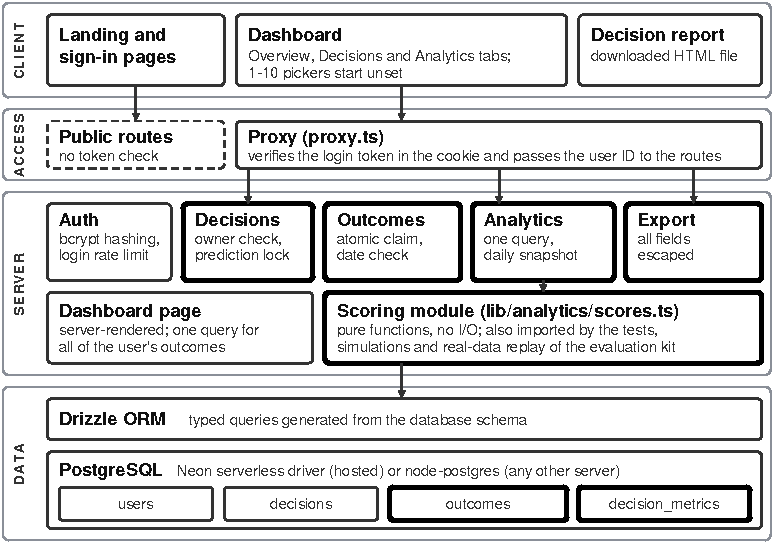
\includegraphics[width=\textwidth]{Fig1.pdf}
\caption{Architecture of Digital Memory Vault (revised implementation). Boxes show components in the client, access, server and data layers, and arrows show the direction of requests. Components with a heavier outline differ from the baseline implementation; the dashed box marks public routes, which bypass the token check}\label{fig:arch}
\end{figure}

\subsection{Scoring rules}\label{sec:rules}

Let $R$ be the set of a user's resolved decisions, $n=|R|$, and for decision $i$ let $c_i$ be the stated confidence and $s_i$ the success rating, both integers from 1 to 10. Bars denote means over the set indicated. Table~\ref{tab:rules} defines the four scores under the baseline and the revised rules; all are reported on a 0--100 scale, with ten points per step of error.

\begin{table}[t]
\caption{Baseline and revised scoring rules}\label{tab:rules}
\footnotesize
\begin{tabular}{@{}L{2.0cm}L{4.6cm}L{4.6cm}@{}}
\toprule
Score & Baseline rules & Revised rules\\
\midrule
Decision accuracy & $\frac{1}{n}\sum_{i\in R}\max(0,100-10|c_i-s_i|)$ & unchanged\\
Confidence calibration & $\max(0,100-10|\bar c-\bar s|)$: compares two overall means & $\max(0,100-10E_c)$, $E_c=\sum_k \frac{n_k}{n}|\bar c_k-\bar s_k|$ over groups $k$ of equal stated confidence\\
Risk calibration & mean of $10\bar s_{\text{high}}$ and $10\bar s_{\text{low}}$; confidence and medium risk ignored & $\max(0,100-10E_r)$, $E_r=\sum_g \frac{n_g}{n}|\bar c_g-\bar s_g|$ over $g\in\{$low, medium, high$\}$\\
Emotional bias & per decision, pending included: 40 if stressed, pressured or uncertain, plus 10 per warning word found as a substring of the reflection, capped at 100; mean over decisions & as baseline, but excited also scores 40, words match whole words and inflections only, and a word preceded within three words by a negation is ignored\\
\midrule
Supporting values & over- and underconfidence rates: share of decisions with $c_i>s_i+1$ and $c_i<s_i-1$ & unchanged; also signed gap $\bar c-\bar s$, $E_c$, $E_r$, gap per risk level, and a flag when $n<\MinimumHistory$\\
\botrule
\end{tabular}
\tabnote{$c_i$, stated confidence of decision $i$; $s_i$, its success rating; $n$, number of resolved decisions; $E_c$ and $E_r$, calibration errors in steps of the 1--10 scale.}
\end{table}

$E_c$ is the expected calibration error of a reliability diagram whose bins are the ten confidence values, expressed in steps \cite{naeini2015}, and $E_r$ is the corresponding calibration error within risk levels \cite{kleinberg2017}. By the triangle inequality both are at least $|\bar c-\bar s|$, so the revised rules never rate a user as better calibrated than the baseline rules do. The twelve warning words are rushed, pressured, anxious, overconfident, doubt, reactive, panic, fear, desperate, impulsive, hasty and regret. In the revised implementation the rules live in a pure module without input or output, which the API, the tests and every offline experiment import, so the code that is evaluated is the code that runs.

Table~\ref{tab:worked} applies both sets of rules to ten illustrative decisions entered through the application. The two high-risk decisions were stated with confidence 9 and 8 and rated 3 and 4. The baseline risk calibration score of \BaseWorkedriskCalibrationScore{} does not register this mismatch, because it never reads confidence; the revised score is \RevWorkedriskCalibrationScore{} and the revised implementation reports a gap of five steps in the high-risk group. The baseline confidence calibration score of \BaseWorkedconfidenceCalibrationScore{} reflects only that mean confidence and mean success are close, although four decisions were overconfident and two underconfident by more than one step.

\begin{table}[t]
\caption{Worked example: ten illustrative decisions (not user data) and the scores returned by the application under the baseline and the revised rules}\label{tab:worked}
\footnotesize
\begin{tabular}{@{}rL{4.6cm}llcc@{}}
\toprule
\# & Decision & Risk & State & Confidence & Success\\
\midrule
1 & Accept internship offer & medium & calm & 8 & 9\\
2 & Buy a laptop on instalments & low & excited & 7 & 7\\
3 & Launch feature without user testing & high & pressured & 9 & 3\\
4 & Join a morning gym batch & low & calm & 6 & 8\\
5 & Move to a shared flat & medium & uncertain & 7 & 5\\
6 & Switch database provider mid-sprint & high & stressed & 8 & 4\\
7 & Apply for a hackathon & medium & calm & 5 & 8\\
8 & Invest savings in an index fund & medium & calm & 6 & 6\\
9 & Hire a freelance designer & medium & excited & 9 & 5\\
10 & Start a weekend course & low & calm & 7 & 8\\
\botrule
\end{tabular}

\smallskip
\begin{tabular}{@{}lcccccc@{}}
\toprule
Rules & DA & CC & RC & EB & Over (\%) & Under (\%)\\
\midrule
Baseline & \BaseWorkeddecisionAccuracyScore & \BaseWorkedconfidenceCalibrationScore & \BaseWorkedriskCalibrationScore & \BaseWorkedemotionalBiasScore & \BaseWorkedoverconfidenceRate & \BaseWorkedunderconfidenceRate\\
Revised & \RevWorkeddecisionAccuracyScore & \RevWorkedconfidenceCalibrationScore & \RevWorkedriskCalibrationScore & \RevWorkedemotionalBiasScore & \RevWorkedoverconfidenceRate & \RevWorkedunderconfidenceRate\\
\botrule
\end{tabular}
\tabnote{DA, decision accuracy; CC, confidence calibration; RC, risk calibration; EB, emotional bias; Over and Under, over- and underconfidence rates. Reflections of decisions 3, 5, 6 and 9 contain warning words (``rushed''; ``doubt''; ``panic'', ``hasty''; ``impulsive'', ``regret''). Confidence and success are on 1--10 scales.}
\end{table}

\section{Evaluation method}\label{sec:method}

Figure~\ref{fig:approach} summarises the approach. Each kind of evidence comes with its own oracle, the thing that decides whether a result is right. The scoring experiments run on the scoring rules as pure functions; a differential check connects them to the running application.

\begin{figure}[t]
\centering
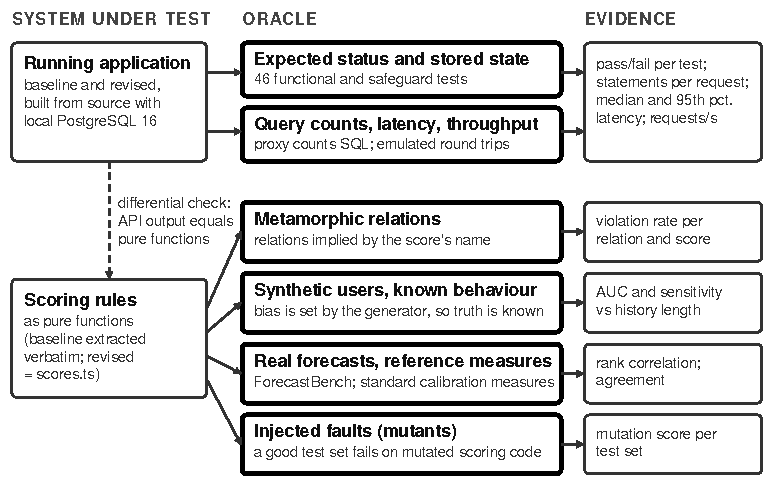
\includegraphics[width=\textwidth]{Fig2.pdf}
\caption{Validation approach. Left: the two forms in which each implementation is tested. Middle: the oracle that decides each verdict. Right: the evidence each produces. The dashed arrow is the differential check, which confirms that the pure scoring functions return exactly what the running application returns}\label{fig:approach}
\end{figure}

\subsection{Implementations and environment}

The artefact contains both implementations as source: the baseline (Next.js 16.1.6) and the revised implementation (Next.js 16.3.8). A script copies each, installs its own locked dependencies, creates a fresh database, builds the application with \texttt{next build} and starts it with \texttt{next start}. All measurements were taken in one run on a Linux machine (Ubuntu 24.04) with two virtual CPUs (Intel Xeon, 2.8\,GHz), 7.8\,GB of memory, Node.js 22.22 and PostgreSQL 16.15. The application servers and the database were pinned to the first CPU and the test clients to the second. The hosted Neon database used in production is not reachable from an isolated machine, so both implementations used the node-postgres driver against the local server; the revised implementation supports both drivers, while the baseline needed a seven-line substitute client file. Section~\ref{sec:net} emulates network round trips explicitly.

\subsection{Functional and safeguard tests}\label{sec:functests}

A Node.js script sends real HTTP requests and compares each response, and where needed the database state, with a predefined expectation. Tests TC01--TC33 cover authentication, route protection, access control between two users, decision logging, outcome recording, analytics and report export. Safeguard tests TC34--TC46 check that each prediction field is locked once an outcome exists, that an outcome cannot be dated before its decision was logged, that ten simultaneous outcome submissions for one decision store exactly one outcome, that every user-supplied field of the report is escaped, that one user cannot edit another's decision, that repeated analytics requests on one day store at most one snapshot, and three scoring relations from Section~\ref{sec:mr} checked through the API.

\subsection{Performance}\label{sec:net}

For each endpoint we measured the response time at the client over 30 sequential requests (20 for registration and login) and report the median and 95th percentile. To see how latency scales, we created users holding 10, 50, 100, 250, 500 and 1,000 resolved decisions, inserted with one SQL statement per table, and measured the analytics endpoint and the dashboard page over 30 requests each after a warm-up request. A small TCP proxy between application and database counted the SQL statements behind each request by parsing the PostgreSQL wire protocol, and could delay every packet in each direction to emulate a round-trip time (RTT) of 0, 2, 5, 10 or 20\,ms. With all four application instances and both proxies running, responses through the proxy were slower than direct ones by a further \ProxyOffsetMin{} to \ProxyOffsetMax{}\,ms at zero added delay, more than the proxy adds in isolation (about 0.1\,ms per query); we therefore compare the implementations by how their latency increases with RTT, not by absolute values. Under load, ten concurrent clients requested the analytics endpoint for 20 seconds for a user with 100 and with 500 decisions. Finally, we audited production dependencies with \texttt{npm audit}.

\subsection{Score validity}

\subsubsection{Metamorphic relations}\label{sec:mr}

Table~\ref{tab:mrdef} lists the relations. MR1--MR3 express what a calibration score must do when confidence is distorted in a known way; MR4--MR6 are invariances that any score computed from a set of independent decisions must have; MR7--MR9 concern the emotional-bias score's text matching. Source histories were generated with 12 to 60 decisions in which confidence equalled the success rating, so the follow-up distortion was the only source of miscalibration. Each relation was checked on \MRSources{} generated source histories for the baseline and the revised rules, and we report the share of sources on which it was violated.

\begin{table}[t]
\caption{Metamorphic relations. A source history is transformed into a follow-up history, and the scores of the two must satisfy the stated relation}\label{tab:mrdef}
\footnotesize
\begin{tabular}{@{}lL{6.2cm}L{3.6cm}@{}}
\toprule
ID & Transformation of the source history & Required relation\\
\midrule
MR1 & Add 2 to every confidence & both calibration scores fall\\
MR2a & Subtract 2 from low-risk and add 2 to high-risk confidences (risk levels mixed at random) & both calibration scores fall\\
MR2b & As MR2a on histories with equal numbers of low- and high-risk decisions, where the two errors cancel in the overall mean & both calibration scores fall\\
MR3 & Shift every confidence by $+3$ instead of $+1$ & both calibration scores lower than with $+1$\\
MR4 & Shuffle the order of decisions & all scores unchanged\\
MR5 & Duplicate the whole history & all scores unchanged\\
MR6 & Add pending decisions & accuracy and calibration unchanged\\
MR7 & Append ``No regrets, not anxious.'' to every reflection & emotional bias does not rise\\
MR8 & Append ``Fearless and undoubtedly sound.'' & emotional bias does not rise\\
MR9 & Replace neutral reflections of calm decisions with ``Panicked and regretted it.'' & emotional bias rises\\
\botrule
\end{tabular}
\tabnote{MR, metamorphic relation.}
\end{table}

\subsubsection{Synthetic users with known behaviour}\label{sec:sim}

Every synthetic decision has an underlying quality $q$ drawn uniformly from 6--9 for low-risk, 4--7 for medium-risk and 2--6 for high-risk decisions; the success rating is $q$ plus normal noise with standard deviation 1.5, rounded and kept within 1--10, and risk levels cycle through low, medium and high. We used two families of reporters. The first, the noisy-reporter design, states as confidence $q$ plus a bias plus normal noise with standard deviation 1, with a calibrated, an overconfident ($+2$), an underconfident ($-2$) and an inconsistent profile ($-3$ on low-risk and $+3$ on high-risk decisions), 25 users of 40 decisions each, entered through the API of each implementation. Because of the added noise, that ``calibrated'' profile is calibrated on average only.

For the power analysis we defined a calibrated reporter as one who states the rounded quality, so that the mean success at each confidence level equals that confidence apart from clamping, and six miscalibrated profiles relative to it: overconfident by one and by two steps, underconfident by two steps, inconsistent by $\pm2$ and $\pm3$ steps by risk level, and noisy, with case-to-case noise of standard deviation 2 and no bias. Users with the same seed share identical outcomes and differ only in reported confidence. For each history length from 5 to 120 decisions and each profile we generated \PowerReps{} miscalibrated and \PowerReps{} calibrated users and computed, for each score, the area under the ROC curve (AUC) for separating the two groups \cite{fawcett2006} and the sensitivity at 95\% specificity: the share of miscalibrated users scoring at or below the highest threshold that flags no more than 5\% of calibrated users. We define the minimum history as the shortest length at which every two-step profile is flagged with at least 80\% sensitivity by at least one revised calibration score.

\subsubsection{Real forecasts}\label{sec:replay}

ForecastBench is a forecasting benchmark that publishes individual forecasts by human superforecasters together with resolutions \cite{karger2025}. From its question set of 21 July 2024 we took every individual superforecaster forecast whose question had resolved to 0 or 1: \ReplayForecasts{} forecasts by \ReplayForecasters{} forecasters with at least 20 resolved forecasts each (median \ReplayMedianPer{}, range \ReplayMinPer{}--\ReplayMaxPer{}); \ReplayBaseRate\% of the questions resolved positively. A probability $p$ was mapped to the application's scale as $c=1+\mathrm{round}(9p)$ and an outcome to a success rating of 10 or 1, so that a forecaster calibrated in probability terms is also calibrated on the 1--10 scale. The question's domain (prediction market, economic data series or event data series) took the place of the risk level as the grouping variable, since it is known when the forecast is made.

For each forecaster we computed the baseline and revised scores and four reference measures from the raw probabilities: ECE over ten equal-width bins \cite{naeini2015}, Murphy's reliability term \cite{murphy1973}, calibration-in-the-large, and the domain-conditional calibration error, the weighted mean absolute gap between mean forecast and outcome frequency within each domain. We report Spearman rank correlations across forecasters with 95\% bootstrap confidence intervals from 2,000 resamples \cite{efron1993}. We then distorted each forecaster's real forecasts in four controlled ways (uniformly $+0.2$ and $-0.2$, $-0.2$ on market and $+0.2$ on event questions, and doubling the log-odds) and counted the forecasters for whom the score moved in the direction opposite to the reference error, that is, fell when the forecaster became less calibrated. Finally, for the \LenForecasters{} forecasters with at least 80 forecasts, we drew 200 random subsets of 10, 20, 40 and 80 forecasts and correlated the score on the subset with the reference measure on the full history.

\subsubsection{Differential check}

The offline experiments use the scoring rules as pure functions: for the revised rules the module the application imports, and for the baseline rules a verbatim extraction from the baseline implementation. To confirm that these functions describe the running applications, the noisy-reporter simulation and a ten-decision worked example (Table~\ref{tab:worked}) were entered through each implementation's API, and every score the API returned was compared with the pure function of the same rules on the same inputs.

\subsection{Test adequacy}

We mutated the revised scoring module with Stryker 9 \cite{stryker} and ran five test sets against every mutant: a worked-example check of the kind developers typically write (the eight values reported for the ten decisions of Table~\ref{tab:worked}, plus an empty history); the same with the metamorphic relations of Table~\ref{tab:mrdef} written as executable tests using fast-check \cite{fastcheck}; the same with ten property-based tests of invariants such as bounds, perfect calibration giving 100, and determinism; that set with example-based unit tests added; and the example-based tests alone. Generated tests ran 100 cases each. Surviving mutants were inspected by hand for equivalence.

\subsection{Use of generative artificial intelligence}\label{sec:ai}

A large language model (Claude, Anthropic) was used to help write the evaluation scripts, the code revisions and the code that renders the figures, and to help draft and edit the text. All scripts were run in the environment described above; the author reviewed the code, its raw output and the complete text, and takes full responsibility for the content. No figure was produced by a generative image model: diagrams are drawn from code and charts are plotted from measured data.

\section{Revisions}\label{sec:repairs}

Table~\ref{tab:repairs} lists every defect the evaluation found in the baseline implementation, the revision made and the evidence used to verify it. Most revisions are small. Prediction locking compares the request with five protected fields and makes the update conditional on the decision still being pending, so the check and the write are atomic. Outcome recording first claims the decision with a single conditional update from pending to resolved, which only one concurrent request can win, and a unique index on the outcome's decision identifier enforces one outcome per decision in the database itself. Analytics and the dashboard read decisions and outcomes with one joined query, and snapshots are upserted on a unique key of user and day. The interface was revised too: the 1--10 ratings now start unset instead of at 7, to avoid anchoring \cite{tversky1974}, the outcome form asks optionally for a separate rating of the decision's quality, and the analytics view marks the calibration scores as provisional below \MinimumHistory{} resolved decisions.

\begin{table}[t]
\caption{Defects found in the baseline implementation, revisions and how each was verified}\label{tab:repairs}
\footnotesize
\begin{tabular}{@{}L{4.2cm}L{4.4cm}L{2.6cm}@{}}
\toprule
Finding in the baseline & Revision & Verified by\\
\midrule
Confidence, emotional state, risk level, expected outcome and decision date editable after the outcome & Edits rejected with 409; condition and update atomic & TC26, TC34--TC38\\
Outcome may be dated before the decision was logged & Rejected with 400 & TC39\\
Two concurrent submissions store two outcomes & Atomic claim and unique index & TC40\\
Six report fields written unescaped & All user text HTML-escaped; restrictive content policy & TC31, TC41\\
One outcome query per decision & One joined query & statement counts, latency, load\\
A snapshot on every analytics request & One snapshot per user and day & TC43\\
Confidence calibration blind to opposite errors & Per-confidence-level error $E_c$ & TC44, MR2b, power\\
Risk calibration ignores confidence & Per-risk-level error $E_r$ & TC45, MR1--MR3, power\\
Warning words matched as substrings, negations counted & Whole words, inflections, negation window & TC46, MR7--MR9\\
No guidance on history length & Provisional flag below \MinimumHistory{} decisions & power analysis\\
14 dependency advisories, 2 critical & Patched framework and libraries; unused PDF library removed & \texttt{npm audit}\\
\botrule
\end{tabular}
\tabnote{TC, functional test case (Section~\ref{sec:functests}); MR, metamorphic relation (Table~\ref{tab:mrdef}); power, detection-power simulation (Section~\ref{sec:sim}).}
\end{table}

\section{Results}\label{sec:results}

\subsection{RQ1: Integrity and security}\label{sec:functional}

The baseline passed \BaseFuncCorePassed{} of the 33 core tests and \BaseFuncSafePassed{} of the 13 safeguard tests; the revised implementation passed all 46 (Table~\ref{tab:func}). The failures in the baseline all concern the integrity of the record rather than crashes. The server accepted changes to every prediction field after the outcome was known, so hindsight could rewrite a prediction \cite{fischhoff1975}. It also accepted an outcome dated years before the decision was logged. When ten outcome submissions for one decision arrived together, two were accepted and two outcomes were stored, because both requests passed the pending check before either recorded the outcome \cite{warszawski2017}. All six user-supplied text fields of the report were inserted unescaped, an injection weakness \cite{owasp2021}, and every visit to the analytics view added a snapshot row. Access control held in both implementations: every attempt by one user to read, edit, delete, export or resolve another user's decision returned 404.

\begin{table}[t]
\caption{Functional and safeguard tests passed, by area}\label{tab:func}
\begin{tabular}{@{}lccc@{}}
\toprule
Area & Tests & Passed, baseline & Passed, revised\\
\midrule
Authentication & 9 & 9 & 9\\
Route protection & 4 & 4 & 4\\
Access control & 4 & 4 & 4\\
Decision logging & 8 & 8 & 8\\
Outcome recording & 5 & 3 & 5\\
Prediction integrity & 6 & 1 & 6\\
Analytics & 6 & 2 & 6\\
Report export & 4 & 2 & 4\\
\midrule
Core tests (TC01--TC33) & 33 & 31 & 33\\
Safeguard tests (TC34--TC46) & 13 & 2 & 13\\
Total & 46 & 33 & 46\\
\botrule
\end{tabular}

\tabnote{TC, test case. Core tests TC01--TC33 and safeguard tests TC34--TC46 are described in Section~\ref{sec:functests}.}
\end{table}

The dependency audit found 14 advisories in the baseline production dependencies, two of them critical (in the framework and in an unused PDF library) and one a high-severity SQL-injection advisory in the ORM's handling of identifiers. The revised implementation updated the framework and the affected libraries and removed the unused one; the audit then reported none.

\subsection{RQ2: Performance}

In the baseline, each analytics request issued one statement for the user's decisions, one per decision for its outcome and one to insert the snapshot: \BaseStatementsTwoZero{} statements at 20 decisions, \BaseStatementsOneZeroZero{} at 100 and \BaseStatementsFiveZeroZero{} at 500. The dashboard followed the same pattern. The revised implementation issued \RevStatementsTwoZero{} statements per analytics request and \RevDashStatementsTwoZero{} per dashboard request at every history length. Median analytics latency in the baseline grew almost linearly, from \BaseAnalyticsOneZeroMedian{}\,ms at 10 decisions to \BaseAnalyticsOneZeroZeroZeroMedian{}\,ms at 1,000, while the revised implementation took \RevAnalyticsOneZeroMedian{}\,ms at 10 decisions and \RevAnalyticsOneZeroZeroZeroMedian{}\,ms at 1,000, \AnalyticsReductionOneZeroZeroZero\% lower at 1,000 decisions (Fig.~\ref{fig:perf}a). The dashboard page fell by \DashboardReductionOneZeroZeroZero\% at 1,000 decisions. Every other endpoint answered within \OtherEndpointMax{}\,ms at the median in both implementations, except registration and login, whose \PasswordMin--\PasswordMax\,s is spent almost entirely in bcrypt at cost factor 12 \cite{provos1999}.

\begin{figure}[t]
\centering
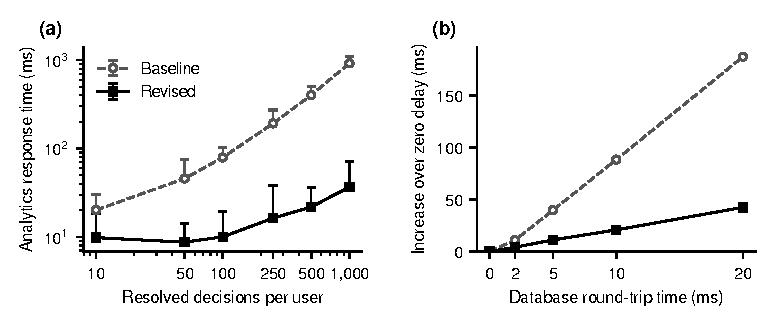
\includegraphics[width=\textwidth]{Fig3.pdf}
\caption{Analytics response time. (a) Median against the number of resolved decisions per user; whiskers extend to the 95th percentile of 30 requests. (b) Increase in median response time over its value with no added delay, against the emulated database round-trip time, for a user with 100 decisions (20 requests per point). Circles on dashed lines show the baseline and squares on solid lines the revised implementation; both axes in (a) are logarithmic}\label{fig:perf}
\end{figure}

The gap widens with distance to the database (Fig.~\ref{fig:perf}b). Each additional millisecond of round-trip time added about \BaseRttSlope{}\,ms to a baseline analytics request at 100 decisions, whose 102 statements run at most ten at a time through the connection pool, against \RevRttSlope{}\,ms for the revised implementation. Under ten concurrent clients (Table~\ref{tab:load}), the revised implementation sustained \LoadGainOneZeroZero{} times the throughput of the baseline at 100 decisions and \LoadGainFiveZeroZero{} times at 500, where the baseline completed only \BaseLoadFiveZeroZeroThroughput{} requests per second. Neither implementation returned an error. Snapshot growth was bounded too: after 31 analytics requests on one day, a user of the baseline held \BaseSnapshotsOneZeroZero{} snapshots and a user of the revised implementation \RevSnapshotsOneZeroZero{}.

\begin{table}[t]
\caption{Analytics endpoint under ten concurrent clients for 20 seconds}\label{tab:load}
\begin{tabular}{@{}llrrrrr@{}}
\toprule
Decisions & Implementation & Requests & Requests/s & Median (ms) & 95th pct.\ (ms) & Errors\\
\midrule
100 & Baseline & 196 & 9.8 & 1,025.0 & 1,236.9 & 0\\
100 & Revised & 2,584 & 129.2 & 71.7 & 109.6 & 0\\
500 & Baseline & 49 & 2.5 & 4,744.9 & 5,124.7 & 0\\
500 & Revised & 1,074 & 53.7 & 175.7 & 266.1 & 0\\
\botrule
\end{tabular}

\tabnote{pct., percentile. Response times were measured at the client.}
\end{table}

\subsection{RQ3: Score validity}\label{sec:simres}

\paragraph{Differential check.} Every score that the running applications returned for the 100 simulated users and the worked example equalled the pure function of the same rules on the same inputs: \BaseDiffMismatches{} of \BaseDiffCompared{} values differed for the baseline and \RevDiffMismatches{} of \RevDiffCompared{} for the revised implementation. Under the baseline rules, the mean risk calibration score was \BaseSimCalibratedriskCalibrationScore{} for every profile, as the rule's definition predicts when outcomes are shared. The offline results below therefore describe what the applications compute.

\paragraph{Metamorphic relations.} Table~\ref{tab:mr} shows the violation rates. The baseline risk calibration score violated MR1, MR2a, MR2b and MR3 on every source history: since it never reads confidence, no distortion of confidence can lower it. Its confidence calibration score detected uniform shifts, but on balanced histories, where low- and high-risk errors cancel in the mean, it violated MR2b every time. Its emotional-bias score rose when ``No regrets, not anxious.'' or ``Fearless'' was added. The revised implementation satisfied every relation, with one exception: in \MRMRTwobrevisedconfidenceCalibrationScore\% of balanced sources, the opposite errors landed on the same confidence level and cancelled within that group, so the confidence calibration score did not fall. The risk calibration score, which groups by risk level, caught all of those cases. Both sets of rules satisfied the invariances MR4--MR6.

\begin{table}[t]
\caption{Share of \MRSources{} source histories on which each metamorphic relation was violated (\%), by rules and score\textsuperscript{\dag}}\label{tab:mr}
\footnotesize
\begin{tabular}{@{}lcccccccc@{}}
\toprule
 & \multicolumn{4}{c}{Baseline rules} & \multicolumn{4}{c}{Revised rules}\\
\cmidrule(lr){2-5}\cmidrule(l){6-9}
Relation & DA & CC & RC & EB & DA & CC & RC & EB\\
\midrule
MR1 & -- & 0 & 100 & -- & -- & 0 & 0 & --\\
MR2a & -- & 14.2 & 100 & -- & -- & 0 & 0 & --\\
MR2b & -- & 100 & 100 & -- & -- & 0.1 & 0 & --\\
MR3 & -- & 0 & 100 & -- & -- & 0 & 0 & --\\
MR4 & 0 & 0 & 0 & 0 & 0 & 0 & 0 & 0\\
MR5 & 0 & 0 & 0 & 0 & 0 & 0 & 0 & 0\\
MR6 & 0 & 0 & 0 & -- & 0 & 0 & 0 & --\\
MR7 & -- & -- & -- & 100 & -- & -- & -- & 0\\
MR8 & -- & -- & -- & 100 & -- & -- & -- & 0\\
MR9 & -- & -- & -- & 0 & -- & -- & -- & 0\\
\botrule
\end{tabular}

\tabnote{\textsuperscript{\dag}CC, confidence calibration; RC, risk calibration; DA, decision accuracy; EB, emotional bias. A dash means the relation does not apply to the score.}
\end{table}

\paragraph{Simulated users.} Table~\ref{tab:sim} shows the noisy-reporter simulation under both sets of rules. In the baseline the inconsistent profile, whose users misjudged every low- and high-risk decision by three steps, received the same confidence calibration score as the calibrated profile (\BaseSimInconsistentconfidenceCalibrationScore{} and \BaseSimCalibratedconfidenceCalibrationScore{}), and risk calibration did not vary at all. In the revised implementation the inconsistent profile scored \RevSimInconsistentconfidenceCalibrationScore{} for confidence calibration and \RevSimInconsistentriskCalibrationScore{} for risk calibration, against \RevSimCalibratedconfidenceCalibrationScore{} and \RevSimCalibratedriskCalibrationScore{} for the calibrated profile. The calibrated profile's revised confidence calibration score of \RevSimCalibratedconfidenceCalibrationScore{} rather than 100 is itself informative: that profile adds case-to-case noise to its confidence, which a reliability diagram correctly shows as overconfidence at the extremes, while the baseline comparison of means could not see it.

\begin{table}[t]
\caption{Noisy-reporter simulation: mean (SD) over 25 users of 40 decisions per profile. All profiles share identical outcomes}\label{tab:sim}
\footnotesize
\begin{tabular}{@{}lrcccccc@{}}
\toprule
 & Mean gap & Accuracy & \multicolumn{2}{c}{Baseline rules} & \multicolumn{2}{c}{Revised rules}\\
\cmidrule(lr){4-5}\cmidrule(l){6-7}
Profile & (steps) & (both) & CC & RC & CC & RC\\
\midrule
Calibrated & 0.0 & 86.2 (1.8) & 98.2 (1.4) & 57.7 (2.9) & 93.3 (1.6) & 97.0 (1.4)\\
Overconfident & 1.9 & 79.2 (2.4) & 81.4 (2.5) & 57.7 (2.9) & 81.1 (2.4) & 81.4 (2.5)\\
Underconfident & $-$1.9 & 78.4 (1.9) & 80.6 (2.4) & 57.7 (2.9) & 80.3 (2.4) & 80.6 (2.4)\\
Inconsistent & $-$0.1 & 75.1 (2.1) & 98.2 (1.8) & 57.7 (2.9) & 82.0 (3.4) & 79.0 (2.0)\\
\botrule
\end{tabular}

\tabnote{CC, confidence calibration; RC, risk calibration; SD, standard deviation. Mean gap is mean confidence minus mean success rating; accuracy is identical under both sets of rules.}
\end{table}

Figure~\ref{fig:power} shows detection power by history length. The baseline risk calibration score had an AUC of 0.50 for every profile and length, no better than chance. Its confidence calibration score never exceeded an AUC of about 0.6 for inconsistent users, however long the history, and was little better for noisy users. The revised risk calibration score separated $\pm2$ inconsistent users from calibrated ones with an AUC of \PowIncTwoRevRCNOneZeroAuc{} at 10 decisions and \PowIncTwoRevRCNTwoZeroAuc{} at 20, and its confidence calibration score detected noisy users (\PowNoisyTwoRevCCNTwoZeroAuc{} at 20). Every two-step profile was flagged with at least 80\% sensitivity at 95\% specificity by \MinimumHistory{} decisions; the revised implementation uses this threshold to mark scores as provisional. The revision has a cost: for a uniform bias of one step, the baseline comparison of means is the more efficient test, reaching \PowOverOneBaseCCNTwoZeroSens\% sensitivity at 20 decisions against \PowOverOneRevRCNTwoZeroSens\% for the revised better score, because grouping spends information on detecting patterns that a uniform shift does not have. The revised implementation still reports the signed mean gap alongside the scores, so that information is not lost to the user.

\begin{figure}[t]
\centering
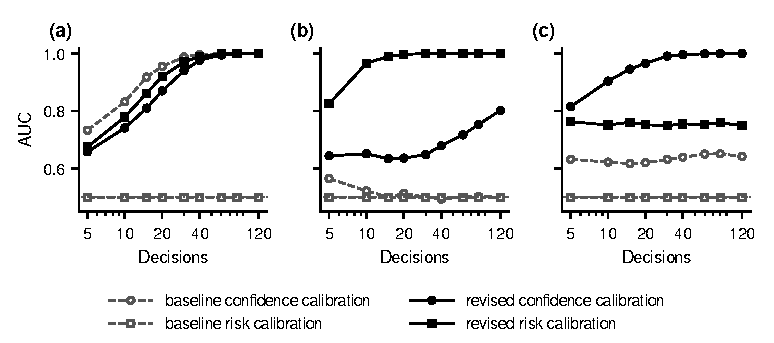
\includegraphics[width=\textwidth]{Fig4.pdf}
\caption{Detection power against history length: area under the ROC curve for separating \PowerReps{} miscalibrated from \PowerReps{} calibrated synthetic users with identical outcomes, for (a) a uniform one-step overconfidence, (b) $\pm2$ steps of risk-dependent inconsistency and (c) case-to-case noise with standard deviation 2. Open markers on dashed lines show baseline scores and filled markers on solid lines revised scores; circles mark confidence calibration and squares risk calibration. An AUC of 0.5 is chance}\label{fig:power}
\end{figure}

\paragraph{Real forecasts.} The \ReplayForecasters{} superforecasters were well calibrated as a group (pooled ECE \ReplayEce{}, Brier score \ReplayBrier{}), but individuals varied (Fig.~\ref{fig:replay}). Table~\ref{tab:replay} shows how each score related to the reference measures. The revised confidence calibration score correlated strongly with ECE ($\rho=$ \RhoB{}) and with Murphy's reliability term (\RhoD{}); the baseline correlated only moderately (\RhoA{}, \RhoC{}), and almost perfectly with the absolute calibration-in-the-large (\RhoE{}), which is all it measures. The revised risk calibration score correlated with the domain-conditional calibration error at \RhoG{}. The baseline showed no relation to it (\RhoF{}, interval spanning zero) and instead tracked how often each forecaster's questions resolved positively (\RhoH{}): it measures how things turned out, not calibration.

\begin{table}[t]
\caption{Spearman correlation between application scores and reference calibration measures across \ReplayForecasters{} superforecasters, with 95\% bootstrap confidence intervals. Because the scores are high when calibration is good and the reference errors are high when it is bad, a valid score correlates negatively with its reference error}\label{tab:replay}
\footnotesize
\begin{tabular}{@{}L{4.0cm}L{3.6cm}rl@{}}
\toprule
Score & Reference measure & $\rho$ & 95\% CI\\
\midrule
Baseline confidence calibration & ECE & $-$0.42 & [$-$0.69, $-$0.10]\\
Revised confidence calibration & ECE & $-$0.91 & [$-$0.96, $-$0.81]\\
Baseline confidence calibration & reliability & $-$0.47 & [$-$0.70, $-$0.15]\\
Revised confidence calibration & reliability & $-$0.80 & [$-$0.90, $-$0.63]\\
Baseline confidence calibration & $|$calibration-in-the-large$|$ & $-$0.96 & [$-$0.98, $-$0.91]\\
Baseline risk calibration & domain calibration error & $-$0.08 & [$-$0.38, 0.23]\\
Revised risk calibration & domain calibration error & $-$0.96 & [$-$0.98, $-$0.91]\\
Baseline risk calibration & outcome base rate & 0.51 & [0.21, 0.72]\\
Revised risk calibration & outcome base rate & $-$0.26 & [$-$0.52, 0.06]\\
\botrule
\end{tabular}

\tabnote{$\rho$, Spearman rank correlation; CI, confidence interval; ECE, expected calibration error.}
\end{table}

\begin{figure}[t]
\centering
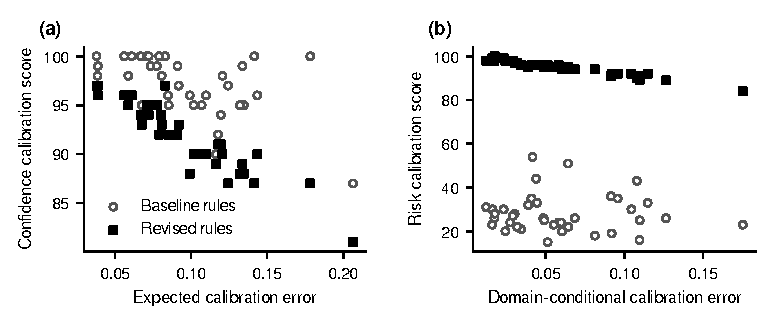
\includegraphics[width=\textwidth]{Fig5.pdf}
\caption{Application scores against reference measures for \ReplayForecasters{} superforecasters. (a) Confidence calibration against expected calibration error (ECE); (b) risk calibration against domain-conditional calibration error. Open circles show the baseline rules and filled squares the revised rules; each forecaster appears once under each}\label{fig:replay}
\end{figure}

The controlled distortions of the real forecasts (Table~\ref{tab:dist}) tell the same story. The baseline risk calibration score did not change for any forecaster under any distortion. Under uniform shifts, both implementations' confidence calibration scores agreed with the reference for most forecasters, the baseline slightly more often under underconfidence (\DistDTwoBaseCC\% against \DistDTwoRevCC\%), in line with the power analysis. Under opposite errors by domain, the revised risk calibration score moved in the right direction for \DistDThreeRevRC\% of forecasters and the baseline confidence calibration score for \DistDThreeBaseCC\%. Doubling the log-odds was the hardest distortion for each of the other scores, probably because many superforecasters already state extreme probabilities, which doubling changes little on a ten-point scale; the revised confidence calibration score still agreed with the reference for \DistDFourRevCC\% of forecasters against \DistDFourBaseCC\% for the baseline. With fewer forecasts the scores were noisier: on random subsets of 20 forecasts, the revised confidence calibration score correlated with the full-history ECE at \LenTwoZerorevisedcc{}, rising to \LenEightZerorevisedcc{} at 80; for the baseline the figures were \LenTwoZerobaselinecc{} and \LenEightZerobaselinecc{}. With binary outcomes each forecast carries less information than a 1--10 rating, so real histories need more records than the simulation suggests.

\begin{table}[t]
\caption{Share of \ReplayForecasters{} forecasters for whom a score moved in the direction indicated by the reference measure when their real forecasts were distorted (\%). Reference: ECE for D1, D2 and D4; domain-conditional calibration error for D3}\label{tab:dist}
\footnotesize
\begin{tabular}{@{}lL{4.6cm}cccc@{}}
\toprule
 & & \multicolumn{2}{c}{Baseline rules} & \multicolumn{2}{c}{Revised rules}\\
\cmidrule(lr){3-4}\cmidrule(l){5-6}
 & Distortion & CC & RC & CC & RC\\
\midrule
D1 & Uniform overconfidence: $p+0.2$ & 95 & 0 & 100 & 97\\
D2 & Uniform underconfidence: $p-0.2$ & 90 & 0 & 87 & 85\\
D3 & Opposite errors by domain: market $-0.2$, event $+0.2$ & 69 & 0 & 85 & 92\\
D4 & Extremised: logit doubled & 28 & 0 & 62 & 33\\
\botrule
\end{tabular}

\tabnote{CC, confidence calibration; RC, risk calibration; $p$, stated probability; ECE, expected calibration error.}
\end{table}

\subsection{RQ4: Test adequacy}

Stryker generated \MutTotal{} mutants of the revised scoring module (Table~\ref{tab:mut}). The worked-example check killed \MutworkedScore\% of them. Adding the metamorphic tests raised this to \MutmetamorphicScore\%, and adding the property-based tests to \MutpropertyScore\%. Example-based unit tests written in response to the surviving mutants, for instance one per negation word and per inflection, raised the score to \MutfullScore\%. The five mutants that survived all four sets alter the tokenizer in ways that cannot change any result, such as allowing empty tokens, and are equivalent. The example-based tests alone killed the same mutants as the full set, so by this measure the metamorphic and property-based tests added no fault detection once thorough examples existed.

\begin{table}[t]
\caption{Mutation analysis of the revised scoring module (\MutTotal{} mutants)}\label{tab:mut}
\footnotesize
\begin{tabular}{@{}L{6.4cm}rrr@{}}
\toprule
Test set & Killed & Survived & Score (\%)\\
\midrule
Worked-example check & 133 & 67 & 66.5\\
+ metamorphic tests & 147 & 53 & 73.5\\
+ property-based tests & 152 & 48 & 76.0\\
+ example-based unit tests (full suite) & 195 & 5 & 97.5\\
Worked-example check + example-based unit tests only & 195 & 5 & 97.5\\
\botrule
\end{tabular}

\tabnote{Score, killed mutants as a percentage of all mutants.}
\end{table}

That measure misses what the generated tests did contribute. During development, a property-based test of order invariance found that an earlier draft of the revised module produced calibration errors that depended on the order of decisions in their last floating-point digits, enough to change a reported score whenever an error fell on a rounding boundary; the module now computes every group statistic from integer sums. Another property, that the over- and underconfidence rates sum to at most 100, failed because the two rates are rounded separately, as in the baseline; the property was corrected to allow one point of rounding. More importantly, the metamorphic relations detect faults that mutation analysis cannot measure: faults in the specification. Every mutant of the revised module is a variant of a valid rule, whereas the baseline risk calibration rule was invalid as written and would have passed any test derived from its own formula, including the worked example.

\section{Discussion}\label{sec:discussion}

\paragraph{A score's name is a specification.} The two invalid baseline scores were not coding errors. Each implemented its formula correctly, and a worked example confirmed it to the last digit. What failed was the formula's relation to its name. Metamorphic relations written from the name (more overconfidence must lower a calibration score, and confidence must matter to a calibration score) exposed both defects on every input, needed no ground truth, and took a few lines each to state. We think this is the cheapest check a developer of any self-tracking score can run, and it belongs alongside the code's unit tests rather than in a later study.

\paragraph{Averages hide inconsistency, and grouping has a price.} The baseline confidence calibration score was a correct measure of calibration-in-the-large and nothing more. Kahneman et al.\ describe the case-to-case variability it could not see as noise and argue that it damages judgment as much as bias does \cite{kahneman2021}. Grouping by confidence and by risk level exposes inconsistency and noise, and on real forecasts it brought the scores in line with the measures forecasters are judged by. It costs some sensitivity to a small uniform bias, and with the ten confidence levels as bins, opposite errors that fall on the same level can still cancel; reporting the signed mean gap and the per-risk gaps next to the scores covers both cases. A score that summarises calibration in one number will always lose something, and the application now says which number to read for which question.

\paragraph{How many decisions are enough.} Self-tracking applications show scores from the first record. The power analysis gives a defensible threshold: with \MinimumHistory{} resolved decisions every two-step miscalibration is flagged reliably in simulation. The replay is a warning that this is optimistic for binary outcomes, where 20 records gave only a moderate correlation with the full-history reference. Marking early scores as provisional is cheap and honest. A person who logs a few consequential decisions a month may need most of a year to reach the threshold, which is worth stating plainly in the interface.

\paragraph{The record needs the same protection as the score.} A prospective decision log protects against hindsight only if the prediction cannot be revised \cite{fischhoff1975}, and the interface alone did not enforce this. The race condition is a reminder that check-then-act code in web applications is unsafe under concurrency even when every individual request is handled correctly \cite{warszawski2017}; a conditional update plus a database constraint closed it. The N+1 query pattern cost little on a local database and much more at realistic round-trip times, which is where a hosted deployment runs.

\paragraph{What the scores still cannot tell.} The success rating mixes judgment with luck, so every score built on it inherits outcome bias \cite{baron1988}. The optional decision-quality rating in the revised implementation lets a user separate the two, but no score uses it yet. The emotional-bias score remains a twelve-word indicator; the revisions made its matching correct, not its construct valid, and validating it would need affect measures that only a study with participants can provide.

\section{Threats to validity}\label{sec:threats}

\textbf{Construct validity.} The simulation encodes one model of how confidence and outcomes relate; the conclusions about detection power hold under that model, and the real-forecast replay was added because of it. In the replay, probabilities and binary outcomes were mapped to the application's 1--10 scales and question domain stood in for risk level. Forecasting questions are not personal decisions, and superforecasters are far better calibrated than most people, which compresses the range of scores and makes the correlations, if anything, conservative. The reference measures are standard but are themselves estimates subject to binning choices.

\textbf{Internal validity.} All timings come from one machine with two virtual CPUs, a local database and an emulated network; absolute values will differ in production. Timings also vary between runs on the same hardware, which is why both implementations were measured in the same run. The tests and relations were written by the developers of the system, and some tests were written after the defects were known; mutation analysis and the replay against independent reference measures limit, but do not remove, that bias. The use of a language model to write evaluation code (Section~\ref{sec:ai}) is mitigated by the differential check and by the published scripts and raw results.

\textbf{External validity.} No real users of the application took part, so we cannot say how people will use the scores or whether seeing them improves calibration, as feedback does for forecasters \cite{moore2017}. The study covers one application. The functional tests cover common cases rather than the full attack surface, and no independent security audit was performed.

\textbf{Conclusion validity.} The replay rests on \ReplayForecasters{} forecasters, and the bootstrap intervals in Table~\ref{tab:replay} are correspondingly wide; the conclusions drawn from it concern clear differences between the baseline and revised rules, not precise values. Simulation results use \PowerReps{} users per cell and fixed seeds and are exactly reproducible.

\section{Conclusion}\label{sec:conclusion}

Digital Memory Vault records personal decisions as predictions and scores them against their outcomes. Testing the code that computed its scores was not enough: two of the four scores computed their formulas correctly and still did not measure what their names claimed. Metamorphic relations derived from the names exposed both defects without any ground truth, simulation with known behaviour showed what each score could detect and after how many decisions, and real forecasts confirmed that the revised scores agree with established calibration measures where the baseline scores did not. The same evaluation found, and verified revisions for, editable predictions, a race that duplicated outcomes, unescaped report fields, a query pattern whose cost grew with every decision, and vulnerable dependencies. Scoring rules in self-tracking software are measurement instruments, and they can and should be tested as rigorously as the code that computes them. The next steps are a study with real users to learn whether the revised scores improve their calibration over time, and validation of the emotional-bias indicator against measured affect.

\section*{References}
\begingroup\small
\renewcommand{\section}[2]{}
\begin{thebibliography}{99}
\bibitem{barr2015} Barr ET, Harman M, McMinn P, Shahbaz M, Yoo S. The oracle problem in software testing: a survey. \emph{IEEE Transactions on Software Engineering} 2015; \textbf{41}(5): 507--525. DOI: 10.1109/TSE.2014.2372785.
\bibitem{chen1998} Chen TY, Cheung SC, Yiu SM. Metamorphic testing: a new approach for generating next test cases. \emph{Technical Report HKUST-CS98-01}, Department of Computer Science, Hong Kong University of Science and Technology: Hong Kong, 1998. Reprinted as arXiv:2002.12543, 2020.
\bibitem{chen2018} Chen TY, Kuo FC, Liu H, Poon PL, Towey D, Tse TH, Zhou ZQ. Metamorphic testing: a review of challenges and opportunities. \emph{ACM Computing Surveys} 2018; \textbf{51}(1): 1--27. DOI: 10.1145/3143561.
\bibitem{segura2016} Segura S, Fraser G, Sanchez AB, Ruiz-Cort\'es A. A survey on metamorphic testing. \emph{IEEE Transactions on Software Engineering} 2016; \textbf{42}(9): 805--824. DOI: 10.1109/TSE.2016.2532875.
\bibitem{brier1950} Brier GW. Verification of forecasts expressed in terms of probability. \emph{Monthly Weather Review} 1950; \textbf{78}(1): 1--3. DOI: 10.1175/1520-0493(1950)078<0001:VOFEIT>2.0.CO;2.
\bibitem{murphy1973} Murphy AH. A new vector partition of the probability score. \emph{Journal of Applied Meteorology} 1973; \textbf{12}(4): 595--600. DOI: 10.1175/1520-0450(1973)012<0595:ANVPOT>2.0.CO;2.
\bibitem{lichtenstein1982} Lichtenstein S, Fischhoff B, Phillips LD. Calibration of probabilities: the state of the art to 1980. In \emph{Judgment under Uncertainty: Heuristics and Biases}, Kahneman D, Slovic P, Tversky A (eds.). Cambridge University Press: Cambridge, 1982; 306--334.
\bibitem{moore2008} Moore DA, Healy PJ. The trouble with overconfidence. \emph{Psychological Review} 2008; \textbf{115}(2): 502--517. DOI: 10.1037/0033-295X.115.2.502.
\bibitem{moore2017} Moore DA, Swift SA, Minster A, Mellers B, Ungar L, Tetlock P, Yang HHJ, Tenney ER. Confidence calibration in a multiyear geopolitical forecasting competition. \emph{Management Science} 2017; \textbf{63}(11): 3552--3565. DOI: 10.1287/mnsc.2016.2525.
\bibitem{mellers2014} Mellers B, Ungar L, Baron J, Ramos J, Gurcay B, Fincher K, Scott SE, Moore D, Atanasov P, Swift SA, Murray T, Stone E, Tetlock PE. Psychological strategies for winning a geopolitical forecasting tournament. \emph{Psychological Science} 2014; \textbf{25}(5): 1106--1115. DOI: 10.1177/0956797614524255.
\bibitem{naeini2015} Pakdaman Naeini M, Cooper GF, Hauskrecht M. Obtaining well calibrated probabilities using Bayesian binning. In \emph{Proceedings of the 29th AAAI Conference on Artificial Intelligence}. AAAI Press: Austin, 2015; 2901--2907. DOI: 10.1609/aaai.v29i1.9602.
\bibitem{guo2017} Guo C, Pleiss G, Sun Y, Weinberger KQ. On calibration of modern neural networks. In \emph{Proceedings of the 34th International Conference on Machine Learning}, PMLR 70. PMLR: Sydney, 2017; 1321--1330.
\bibitem{kleinberg2017} Kleinberg J, Mullainathan S, Raghavan M. Inherent trade-offs in the fair determination of risk scores. In \emph{8th Innovations in Theoretical Computer Science Conference (ITCS 2017)}, LIPIcs 67. Schloss Dagstuhl: Dagstuhl, 2017; 43:1--43:23. DOI: 10.4230/LIPIcs.ITCS.2017.43.
\bibitem{li2010} Li I, Dey A, Forlizzi J. A stage-based model of personal informatics systems. In \emph{Proceedings of the SIGCHI Conference on Human Factors in Computing Systems}. ACM: New York, 2010; 557--566. DOI: 10.1145/1753326.1753409.
\bibitem{epstein2020} Epstein DA, Caldeira C, Figueiredo MC, Lu X, Silva LM, Williams L, Lee JH, Li Q, Ahuja S, Chen Q, Dowlatyari P, Hilby C, Sultana S, Eikey EV, Chen Y. Mapping and taking stock of the personal informatics literature. \emph{Proceedings of the ACM on Interactive, Mobile, Wearable and Ubiquitous Technologies} 2020; \textbf{4}(4): 126. DOI: 10.1145/3432231.
\bibitem{fischhoff1975} Fischhoff B. Hindsight $\neq$ foresight: the effect of outcome knowledge on judgment under uncertainty. \emph{Journal of Experimental Psychology: Human Perception and Performance} 1975; \textbf{1}(3): 288--299. DOI: 10.1037/0096-1523.1.3.288.
\bibitem{baron1988} Baron J, Hershey JC. Outcome bias in decision evaluation. \emph{Journal of Personality and Social Psychology} 1988; \textbf{54}(4): 569--579. DOI: 10.1037/0022-3514.54.4.569.
\bibitem{lerner2015} Lerner JS, Li Y, Valdesolo P, Kassam KS. Emotion and decision making. \emph{Annual Review of Psychology} 2015; \textbf{66}: 799--823. DOI: 10.1146/annurev-psych-010213-115043.
\bibitem{kitchenham1995} Kitchenham B, Pfleeger SL, Fenton N. Towards a framework for software measurement validation. \emph{IEEE Transactions on Software Engineering} 1995; \textbf{21}(12): 929--944. DOI: 10.1109/32.489070.
\bibitem{briand1996} Briand LC, Morasca S, Basili VR. Property-based software engineering measurement. \emph{IEEE Transactions on Software Engineering} 1996; \textbf{22}(1): 68--86. DOI: 10.1109/32.481535.
\bibitem{kaner2004} Kaner C, Bond WP. Software engineering metrics: what do they measure and how do we know? In \emph{Proceedings of the 10th International Software Metrics Symposium (METRICS 2004)}. IEEE: Chicago, 2004.
\bibitem{xie2011} Xie X, Ho JWK, Murphy C, Kaiser G, Xu B, Chen TY. Testing and validating machine learning classifiers by metamorphic testing. \emph{Journal of Systems and Software} 2011; \textbf{84}(4): 544--558. DOI: 10.1016/j.jss.2010.11.920.
\bibitem{claessen2000} Claessen K, Hughes J. QuickCheck: a lightweight tool for random testing of Haskell programs. In \emph{Proceedings of the Fifth ACM SIGPLAN International Conference on Functional Programming}. ACM: New York, 2000; 268--279. DOI: 10.1145/351240.351266.
\bibitem{jia2011} Jia Y, Harman M. An analysis and survey of the development of mutation testing. \emph{IEEE Transactions on Software Engineering} 2011; \textbf{37}(5): 649--678. DOI: 10.1109/TSE.2010.62.
\bibitem{papadakis2019} Papadakis M, Kintis M, Zhang J, Jia Y, Le Traon Y, Harman M. Mutation testing advances: an analysis and survey. \emph{Advances in Computers} 2019; \textbf{112}: 275--378. DOI: 10.1016/bs.adcom.2018.03.015.
\bibitem{chen2014} Chen TH, Shang W, Jiang ZM, Hassan AE, Nasser M, Flora P. Detecting performance anti-patterns for applications developed using object-relational mapping. In \emph{Proceedings of the 36th International Conference on Software Engineering}. ACM: New York, 2014; 1001--1012. DOI: 10.1145/2568225.2568259.
\bibitem{yang2018} Yang J, Yan C, Subramaniam P, Lu S, Cheung A. How not to structure your database-backed web applications: a study of performance bugs in the wild. In \emph{Proceedings of the 40th International Conference on Software Engineering}. ACM: New York, 2018; 800--810. DOI: 10.1145/3180155.3180194.
\bibitem{warszawski2017} Warszawski T, Bailis P. ACIDRain: concurrency-related attacks on database-backed web applications. In \emph{Proceedings of the 2017 ACM International Conference on Management of Data}. ACM: New York, 2017; 5--20. DOI: 10.1145/3035918.3064037.
\bibitem{owasp2021} OWASP Foundation. OWASP Top 10:2021. \url{https://owasp.org/Top10/} [accessed 12 October 2026].
\bibitem{fawcett2006} Fawcett T. An introduction to ROC analysis. \emph{Pattern Recognition Letters} 2006; \textbf{27}(8): 861--874. DOI: 10.1016/j.patrec.2005.10.010.
\bibitem{karger2025} Karger E, Bastani H, Yueh-Han C, Jacobs Z, Halawi D, Zhang F, Tetlock PE. ForecastBench: a dynamic benchmark of AI forecasting capabilities. In \emph{Proceedings of the 13th International Conference on Learning Representations (ICLR 2025)}. Singapore, 2025.
\bibitem{efron1993} Efron B, Tibshirani RJ. \emph{An Introduction to the Bootstrap}. Chapman \& Hall: New York, 1993.
\bibitem{stryker} Stryker Mutator contributors. StrykerJS: mutation testing for JavaScript and TypeScript, version 9.6. \url{https://stryker-mutator.io} [accessed 12 October 2026].
\bibitem{fastcheck} Dubien N. fast-check: property-based testing framework for JavaScript and TypeScript, version 4.10. \url{https://fast-check.dev} [accessed 12 October 2026].
\bibitem{tversky1974} Tversky A, Kahneman D. Judgment under uncertainty: heuristics and biases. \emph{Science} 1974; \textbf{185}(4157): 1124--1131. DOI: 10.1126/science.185.4157.1124.
\bibitem{provos1999} Provos N, Mazi\`eres D. A future-adaptable password scheme. In \emph{Proceedings of the 1999 USENIX Annual Technical Conference, FREENIX Track}. USENIX Association: Monterey, 1999; 81--91.
\bibitem{kahneman2021} Kahneman D, Sibony O, Sunstein CR. \emph{Noise: A Flaw in Human Judgment}. Little, Brown Spark: New York, 2021.
\end{thebibliography}
\endgroup


\section*{Acknowledgments}
The author thanks the Forecasting Research Institute for publishing the ForecastBench datasets under an open licence.

\section*{Supporting information}
Additional supporting information may be found online in the Supporting Information section at the end of this article. \textbf{Supporting Information S1} (zip archive): the source code of the baseline and revised implementations, the evaluation kit, the raw results of the run reported here, every number in the paper as generated macros, and the derived real-forecast dataset.

\end{document}
